%\documentclass[12pt,letterpaper]{article}
%\usepackage{setspace}
%\doublespacing
%\usepackage{iccv}
%\documentclass[10pt,preprint,nocopyrightspace]{sigplanconf}
%\documentclass[9pt]{sig-alternate}
%\documentclass[10pt,preprint]{sigplanconf}
\documentclass[10pt,twocolumn]{sigplanconf}
\usepackage{times}
\usepackage{epsfig}
\usepackage{graphicx}
\usepackage{setspace}
\usepackage{amsmath}
\usepackage{amssymb}
\usepackage{subfigure}
\usepackage{multirow}
\usepackage[linesnumbered,noend,ruled]{algorithm2e}
\usepackage{floatflt}
%\usepackage{floatrow}
%\floatsetup{footposition=caption}
%\newcommand{\subparagraph}{}

%\usepackage[small,compact]{titlesec}
%\usepackage[scriptsize,it]{caption}
%\DeclareCaptionFormat{myformat}{\hrulefill \newline #1#2#3}
%\captionsetup[figure]{format=myformat}

\newcommand{\mybeginlist}{\begin{list}{\labelitemi}{\setlength{\itemindent}{0.0in}}}
\newcommand{\mypar}[1]{\vspace{0.0in}\noindent{\bfseries#1}\hspace{0.5em}}
\newcommand{\myparnoskip}[1]{\noindent{\bfseries #1}\hspace{1em}}
\newcommand{\ie}{\emph{i.e.}, }
\newcommand{\eg}{\emph{e.g.}, }
\newcommand{\etc}{\emph{etc.}}
\newcommand{\etal}{, \emph{et al.}}

\newcommand{\squishlist}{
 \begin{list}{$\bullet$}
  { \setlength{\itemsep}{0pt}
     \setlength{\parsep}{1pt}
     \setlength{\topsep}{1pt}
     \setlength{\partopsep}{0pt}
     \setlength{\leftmargin}{1.0em}
     \setlength{\labelwidth}{1em}
     \setlength{\labelsep}{0.5em} } }

\newcommand{\squishlisttwo}{
 \begin{list}{$\bullet$}
  { \setlength{\itemsep}{0pt}
     \setlength{\parsep}{0pt}
    \setlength{\topsep}{0pt}
    \setlength{\partopsep}{0pt}
    \setlength{\leftmargin}{2em}
    \setlength{\labelwidth}{1.5em}
    \setlength{\labelsep}{0.5em} } }

%\titlespacing{\section}{0pt}{*0}{*0}
%\titlespacing{\subsection}{0pt}{*0}{*0}
%\titlespacing{\subsubsection}{0pt}{*0}{*0}

% vertical space reducers
\newcommand{\mysection}[1]{\vspace{-0.11in}\section{#1}\vspace{-0.09in}}
\newcommand{\mysectionstar}[1]{\vspace{-0.15in}\section*{#1}\vspace{-0.16in}}
\newcommand{\mysubsection}[1]{\vspace{-0.12in}\subsection{#1}\vspace{-0.11in}}
\newcommand{\mysubsectionstar}[1]{\vspace{-0.15in}\subsection*{#1}\vspace{-0.13in}}

\newcommand{\squishend}{
  \end{list}  }

% Include other packages here, before hyperref.

% If you comment hyperref and then uncomment it, you should delete
% egpaper.aux before re-running latex.  (Or just hit 'q' on the first latex
% run, let it finish, and you should be clear).
%\usepackage[pagebackref=true,breaklinks=true,letterpaper=true,colorlinks,bookmarks=false]{hyperref}
%\usepackage[pagebackref=true,breaklinks=true,colorlinks,bookmarks=false]{hyperref}
\usepackage[breaklinks=true,colorlinks,bookmarks=false]{hyperref}

\begin{document}

\titlebanner{}        % These are ignored unless
%\preprintfooter{}   % 'preprint' option specified.

\title{A compiler level intermediate representation based binary analysis and rewriting system}
%\subtitle{}

\authorinfo{}
           
           
\maketitle

%\setcounter{page}{1}
%\vspace*{-9ex}
\begin{abstract}

This paper presents modulo unrolling without unrolling (WU), a method for message aggregation for parallel loops in message passing programs that use affine array accesses in Chapel, a Partitioned Global Address Space (PGAS) parallel programming language. Messages incur a non-trivial run time overhead, a significant component of which is independent of the size of the message. Therefore, aggregating messages improves performance. Our optimization for message aggregation is based on a technique known as modulo unrolling, pioneered by Barua \cite{barua1999maps}, whose purpose was to ensure a statically predictable single tile number for each memory reference for tiled architectures, such as the MIT Raw Machine \cite{waingold1997baring}. Modulo unrolling WU applies to data that is distributed in a cyclic or block-cyclic manner. In this paper, we adapt the aforementioned modulo unrolling technique to the difficult problem of efficiently compiling PGAS languages to message passing architectures. When applied to loops and data distributed cyclically or block-cyclically, modulo unrolling WU can decide when to aggregate messages thereby reducing the overall message count and runtime for a particular loop. Compared to other methods, modulo unrolling WU greatly simplifies the complex problem of automatic code generation of message passing code. It also results in substantial performance improvement compared to the non-optimized Chapel compiler. 

\begin{comment}
This paper presents a loop optimization for message passing programs that use affine array accesses in Chapel, a Partitioned Global Address Space (PGAS) parallel programming language. Each message in Chapel incurs some non-trivial run time overhead. Therefore, aggregating messages improves performance. The optimization is based on a technique known as modulo unrolling, where the locality of any affine array access can be deduced at compile time if the data is distributed in a cyclic or block cyclic fashion. First pioneered by Barua \cite{barua1999maps} for tiled architectures, we adapt modulo unrolling to the problem of compiling PGAS languages to message passing architectures. When applied to loops and data distributed cyclically or block cyclically, modulo unrolling can decide when to aggregate messages thereby reducing the overall message count and run time for a particular loop. Compared to other methods, modulo unrolling greatly simplifies the very complex problem of automatic code generation of message passing code from a PGAS language such as Chapel. It also results in substantial performance improvement compared to the non-optimized Chapel compiler.
\end{comment}

To implement this optimization in Chapel, we modify the leader and follower iterators in the Cyclic and Block Cyclic data distribution modules. Results were collected that compare the performance of Chapel programs optimized with modulo unrolling WU and Chapel programs using the existing Chapel data distributions. Data collected on a ten-locale cluster show that on average, modulo unrolling WU used with Chapel's Cyclic distribution results in 76 percent fewer messages and a 45 percent decrease in runtime for our suite of benchmarks. Similarly, modulo unrolling WU used with Chapel's Block Cyclic distribution results in 72 percent fewer messages and a 52 percent decrease in runtime. 

\end{abstract}



\section{Introduction}\label{s:intro}
Chapel is an emerging parallel language being developed by Cray Inc. with
the goal of improving programmer productivity on large-scale systems as
well as on the desktop. It has been developed with the goal being to a
large extent the  standard HPCesque battery of programs which in the large
majority of cases do not involve heavy string based processing, and up
until recently this held true with the vast majority of HPC applications.

However, with the event of big data, and especially looking at iterative
programs we see that in many cases these programs can
benefit from an in memory MapReduce as demonstrated in \cite{zaharia2010spark},
in which the files data is read in and worked on the node that hosts that data 
- retaining the data on that node until it is told that it is no longer needed - 
and doing MapReduce operations using these nodes.

We assert that Chapel could work quite well in this framework. In this
document we explore how to go about adding MapReduce operations to Chapel as 
well as how this might benefit the user not only in terms of speed, but also 
in terms of user productivity.

%We also explore another approach: a MapReduce-mapreduce type operation in which data
%aggregation is done in the first MapReduce, at the end of which all the data that is
%needed is mapped to different nodes locally in memory, at which point we can then run
%a regular program in parallel over this data. This gives performance improvements not
%only in iterative tasks, but also in tasks that require large amounts of contextual
%information (since the reduce at the end of the first MapReduce can condense and
%give us all the information that we need). Not only does this give us the opportunity to then
%explore greater degrees of parallelism as well as faster communication between nodes,
%but we can also utilize non-standard architectures (GPU, MIC) to our benefit. 
%
%\tz{think: supercomputer hooked up to a Hadoop cluster}

\vspace{-1ex}
\section{Contributions}
%\vspace{-1ex}
\label{sec:contributions}
We have identified the two tasks below as key for translating binaries to compiler IR. We demonstrate the advantages of these two methods through the source-code recovered from a binary corresponding to the example code in Fig~\ref{fig:origCCode}(a).
%shows an example which will be used an an example throughout the following discussion.
%Our techniques for these tasks can be applied to any translation system in general - be it static or dynamic. arguments are 

\noindent $\bullet$ \textbf{Deconstruction of physical stack frames} A source program has an abstract stack representation where the local variables are assumed to be present on the stack but their precise stack layout is not specified. In contrast, a binary program has a fixed (but not explicitly specified) physical stack layout, which is used for allocating local variables as well as for passing the arguments between procedures.
%but where locals and arguments are not listed.The compiler is free to generate any stack layout. 

%(Later in this section, we will create IR symbols for individual stack locations)
To recreate a compiler IR, the physical stack must be deconstructed to individual abstract frames, one per procedure. Since the relative
layout of these frames might change in the rewritten binary, the correct representation requires \emph{all} the arguments (interprocedural accesses through stack pointer) to be recognized and translated to symbols in the IR.
 %layout of these abstract frames might change in the rewritten binary, interprocedural accesses through stack pointer might refer to invalid locations. The correct representation requires \textbf{all} the arguments to be recognized and translated to symbols in the IR.

 %With such an IR, the relative layout of frames might change in the rewritten binary. Consequently, the correctness of physical stack references using the stack pointer from one procedure to a parent or ancestor procedure's frame (common for procedure arguments) no longer holds true. or memory-loaded  This results in undiscovered interprocedural stack accesses, jeopardizing correct recovery of IR. shown (one of many possible) due to the lack of symbolic information

Unfortunately, guaranteeing the static discovery of all the arguments is impossible. Some indirect memory references with run-time-computed addresses might make it impossible for an analysis to statically assign them to a fixed stack location, resulting in undiscovered interprocedural accesses. \emph{Existing frameworks circumvent this problem by preserving the monolithic unmodified stack in the IR, resulting in a low-level IR where no local variables can be added or deleted}.

Some binary analysis tools analyze statically determinable stack accesses to recognize \emph{most} arguments~\cite{gogul04}, aiding limited code understanding. However, the lack of guaranteed discovery of \emph{all} the arguments renders such best-effort techniques insufficient for obtaining a functional IR. Fig~\ref{fig:abstract-stack-diff} shows an example procedure where the first argument \emph{a} can be recognized statically while the second argument \emph{b} is not statically discoverable. In the assembly code, \emph{\&a (esp+20)} is stored to the memory location for \emph{p (esp+8)} (Line 2), which is loaded later to temporary \emph{ecx} (Line 4). The source compiler exploited the layout information (\emph{\&a+4=\&b}) to load \emph{b} by incrementing \emph{p (\&a)} by 4 (Line 5). This is safe since the compiler was able to determine that \emph{p} does not alias \emph{q}. However, the binary framework may not be able to establish this relation, since alias analysis in binaries is less precise. Hence, it has to conservatively assume that the \emph{*q} reference (Line 3) could modify \emph{p} which contained the pointer to \emph{a}. Consequently, the source address at Line 5 is no longer known and argument \emph{b} does not get recognized.

Our analysis in Sec~\ref{sec:deconstructFrame} defines a source-level stack model and checks if the executable conforms to this model. If the model is verified for a procedure, the analysis discovers the arguments statically when possible, but when not possible, embeds run-time checks in IR to maintain the correctness of interprocedural data-flow. Otherwise, stack abstraction is discontinued only in that procedure.
%where a runtime stack is maintained, and stack activation records are created upon procedure entry and destroyed upon exit. of argument data-flow

Fig~\ref{fig:origCCode}(c) demonstrates the impact of abstract stack on the recovered source code. Fig~\ref{fig:origCCode}(b) employs a global pointer \emph{llvm\_ESP}, corresponding to the physical stack frame in the input binary, for interprocedural communication as well as for representing local allocations in each procedure. However, in Fig~\ref{fig:origCCode}(c), the stack pointer disappears; instead, local allocations appear as separate local arrays \emph{llvm\_ESP1} and \emph{llvm\_ESP2} and arguments are passed explicitly.

%Recovering a guaranteed-correct IR gives SecondWrite the advantages of IR listed in section~\ref{sec:intro}, such as unrestricted high-level compiler optimizations and reuse of mature compiler passes. are represented as adjustments of pointer \emph{llvm\_ESP}explicit arguments are  Further, Fig~\ref{fig:origCCode}(c) employs \emph{llvm\_ESP} for interprocedural communication whereas Fig~\ref{fig:origCCode}(b) uses explicit arguments.

\noindent $\bullet$ \textbf{Symbol promotion} Another key challenge we solve is \emph{symbol promotion}, which is the process of safely translating a memory location (or a range of locations) to a symbol in the recovered IR. Existing frameworks do not promote symbols; instead they retain memory locations in their IR~\cite{plto,Diablo1,pintool,dyninst94,newEtch}. Some post-link time optimizers like Ispike~\cite{ispike} promote memory locations to symbols employing the symbol-table information in the object files. However, deployed binaries do not contain symbol information, rendering such solutions unsuitable for our framework.

At first glance, it seems that the well-known methods for variable identification in binaries, such as IDAPro~\cite{ida-pro} and Divine~\cite{reps06}, can be used for symbol promotion. However, this is not the case. The presence of potentially aliasing memory references is a key hindrance to the legal promotion of these identified variables to symbols.
%Variable identification is when binary analysis can discover a variable which is the same as the one defined in the source code. \emph{However, variable identification cannot be used for symbol promotion} because (i) the latter has additional non-aliasing requirements not present in the former; and (ii) symbols recovered need not be the same as the source-code variables. We discuss both below.

IDAPro characterizes statically determinable stack offsets in the program as local variables while Divine divides stack memory region into abstract locations by analyzing indirect memory accesses instructions as well. 
%Divine~\cite{reps06} employs Value Set Analysis (VSA) to aid variable recognition. generating constraints for
%VSA is a combined numeric and pointer analysis which determines an over-approximation of the set of memory addresses as well as the set of integer values that each data object (a register or a memory location) can hold at each program point.  The composition of this stack frame is unknown since the symbolic information is absent in stripped binaries. 

The example in Fig~\ref{fig:ident-prom-diff} illustrates the key limitations of both these methods. When the code is compiled, we obtain a stack frame for \emph{main()} of size 48 bytes (10*4 bytes for array \emph{A[]}, and 4$\times$2 = 8 bytes for the scalars \emph{i} and \emph{x}). The accesses to variables \emph{i} and \emph{x} appear as direct memory references (Lines 3,4,6,9) while the array \emph{A} is accessed using an indirect memory reference (Line 7). Both Divine and IDAPro identify memory locations \emph{(esp+44)(x)} and \emph{(esp+40)(i)} as variables based on the direct references. Since the upper bound for the indirect reference to \emph{A[i]} is statically indeterminable, even Divine does not generate any useful information about this access. Hence, it creates three abstract locations - two scalars of 4 bytes each, and a leftover range of 40 bytes.

\emph{Despite dividing stack memory region into three abstract locations, none of them can be promoted to symbols.} It is impossible to statically prove from the stripped binary that the indirect reference at Line 7 does not alias with references to \emph{i} or \emph{x}. Hence, the promotion of memory locations corresponding to \emph{i} and \emph{x} to symbols would be unsafe since it leads to potentially inconsistent data-flow for underlying memory locations. (Source-level alias analyses often assume that any \emph{A[x]} will access \emph{A[]} within its size. However, such size information is not present in a stripped binary.)
%it is not possible to make this assumption in a binary, since variable size is unknown in absence of symbolic information)
%(Source-level alias analysis methods often assume that A[x] will access A[] within its size, and thus not alias with adjacent variables in the layout. However, it is not possible to make this assumption in the binary, since lacking symbolic information, we do not know what variables are present with what sizes.)

Since identification is inadequate for promotion, we have devised a new algorithm to safely promote a set of memory locations to symbols. It computes a set of non-overlapping promotion lifetimes for each memory location taking into consideration the impact of aliasing memory accesses. Our method is oblivious to the underlying method employed for identifying these locations. The locations can be identified by IDAPro, Divine or through a similar method we use.

Fig~\ref{fig:origCCode}(d) shows the improvement in source code recovery from symbol promotion. Fig~\ref{fig:origCCode}(d) demonstrates the replacement of all access to local array \emph{llvm\_ESP1} and \emph{llvm\_ESP2} in procedures \emph{foo} and \emph{main} respectively by local symbols. As evident, this greatly simplifies the IR and the source code.

%Since identification is inadequate for promotion, we have devised a new promotion method. It identifies possibly aliasing indirect references for each candidate direct reference to be promoted. We divide a procedure into regions, such that there are no aliasing indirect references in that region; hence promotion is safe within the region. To maintain correctness across regions, symbols are loaded from their underlying memory locations upon region entry, and saved upon region exit. In the best case, a region may span an entire function, eliminating the overhead of region-boundary load/stores. Our method to safely promote memory locations to symbols is invariant of the underlying method employed for identifying these locations. The locations can be identified by IDAPro or through Divine.
\noindent {\underline {\textbf{Benefits of abstract stack and symbols}}} The presence of abstract stack and symbols has the following advantages:
\begin{itemize}
\renewcommand{\labelitemi}{\textbf{$\rightarrow$}}
\vspace{-3ex}
\item Improved dataflow analysis since standard dataflow analyses only track symbols and not memory locations.
\item Improved readability of the recovered source-code.
\item The ability to employ source-level transformations without any changes. Advanced transformations like compiler-level parallelization~\cite{ParallelAugust,ParallelSohi} add new local variables as barriers and rely on the recognition of induction variables. Several compile-time security mechanisms like StackGuard~\cite{stackguard} and ProPolice~\cite{propolice1} modify stack layout by placing a \emph{canary} (a memory location) on the stack or by allocating local buffers above other local variables. These methods can be implemented only if the framework supports stack modification and symbol promotion.
\item Efficient reasoning about symbolic memory in case of symbolic execution.
%The inability to perform stack modification and the lack of dataflow analysis of memory locations in existing binary frameworks hinders the direct implementation of such techniques. 
%Further, the absence of enough free registers at the required program points might even make them infeasible. In contrast, we can directly employ the same source-level methods in our rewriter without any changes.between local variables and the return address. Similarly,  changes the stack layout to 
%\item Ability to employ compile-time security defense mechanisms. For example, StackGuard~\cite{stackguard} and ProPolice~\cite{propolice1} modify stack layout by placing a \emph{canary} (a memory location) on the stack or by allocating local buffers above all other local variables. These methods can be implemented only if the framework allows stack modification.

\end{itemize}
 
 %As we explain in Sec~\ref{sec:symExec}, symbol promotion also helps in efficient reasoning about symbolic memory in case of symbolic execution. Further, it improves the applicability of various advanced compiler transformations as explained below.

%The techniques presented in this paper can be applied to any translation system in general - be it static or dynamic. In addition, our method becomes a great platform to statically optimize binaries with future optimizations by other researchers, which may not have been developed yet. We consider this enabling of future methods one of our major contributions, in addition to the run-time improvements in this paper.

%De-constructing the physical stack creates symbols for the stack frame and function arguments. Symbol promotion furthers this process by creating additional symbols within stack frames. The reason symbols help run-time is that dataflow analysis tracks symbols, but not memory locations. Hence every dataflow-based compiler optimization becomes more effective with our symbol-creating methods. This includes standard LLVM optimizations that can be applied to the binary, as well as specialized transformations we have tried, such as automatic parallelization and security enhancement. 
%Examples of how specific advanced optimizations rely on stack modification and symbol promotion are as follows. 

%%\begin{figure}[t]
%\vspace{-0.5in}
%\centering
%\psfig{figure=figures/plots/runtimeFinal.eps,width=5.5in} }
%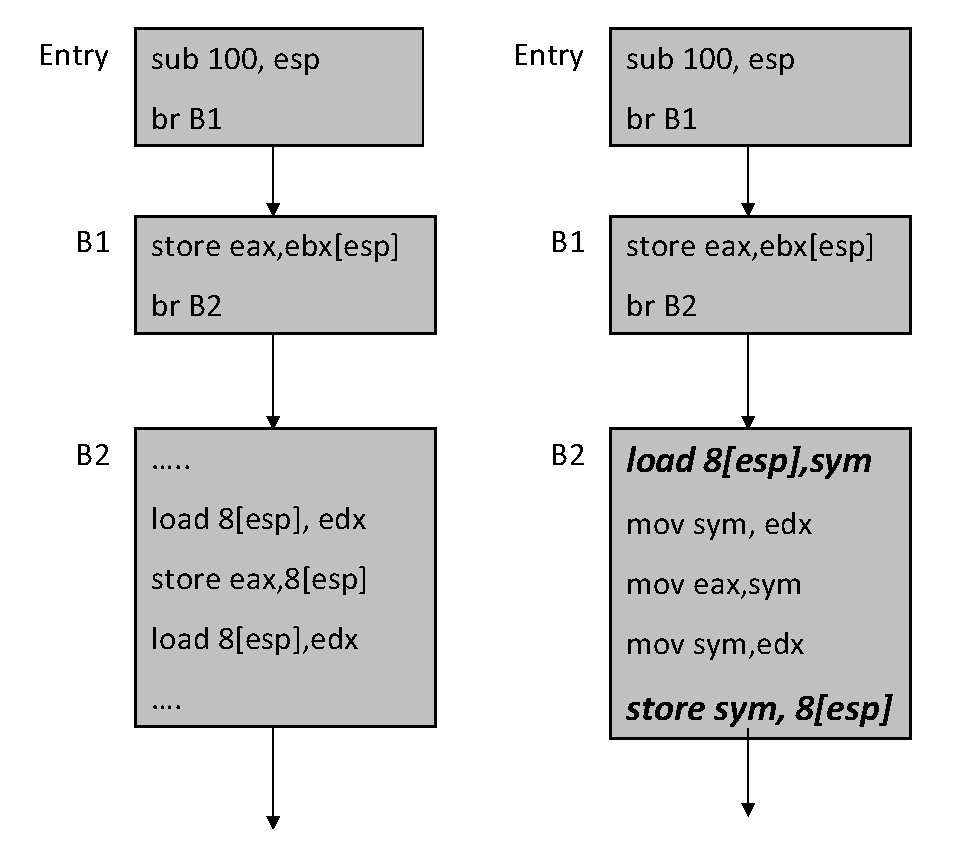
\includegraphics [width=0.5\linewidth] {figures/EPS/cfgex.eps} 
%\tiny{
%\caption { \textit{Stack layout in a binary}}
%}
%\label{fig:stack-layout}
%\end{figure}

\begin{figure}[t]
{
%\begin{minipage}{.5\linewidth}
{
\centering
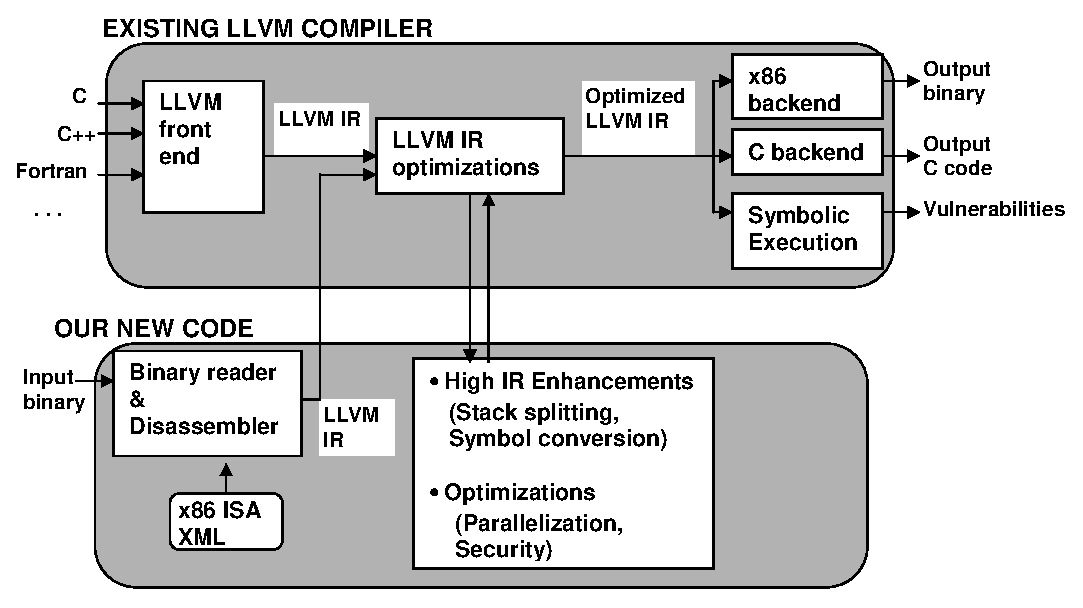
\includegraphics[width=0.7\linewidth]{figures/EPS/flow1.eps}
\caption{\scriptsize{System Flow}}
\label{fig:systemflow}
\vspace{-0.2in}
}
%\end{minipage}
\hfill
%\begin{minipage}{0.3\linewidth}
%{
%\centering
%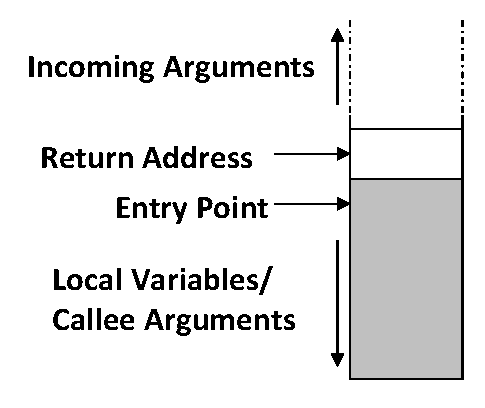
\includegraphics[width=\linewidth]{figures/EPS/stackLayout1.eps} 
%\caption{A typical stack layout}
%\label{fig:stacklayout}
%}
%\end{minipage}
\vspace{-0.2in}
}
\end{figure}

Fig~\ref{fig:systemflow} presents an overview of our framework. SecondWrite produces an initial LLVM IR using custom binary reader modules. The initial IR is enhanced using the above mentioned techniques to obtain an enhanced IR, which can be employed for multiple applications described in Sec~\ref{sec:intro}.

%The frontend module in \emph{SecondWrite} system, consisting of a disassembler and a custom reader module, processes the individual instructions in input executable and generates an initial LLVM IR. This initial representation is devoid of the desired IR features like abstract stack frame and symbols. This initial IR is analyzed to obtain an improved IR which has all the information and features mentioned previously. The standard suite of LLVM optimizations and various new optimization passes can be applied on the above IR to get an optimized IR. The optimized IR is finally passed to the existing LLVM code generator to obtain the rewritten binary. The C backend present in LLVM compiler can be used to obtain C code for better analysis of executables.
%\footnote{Indirect calls and branches occurring in the original binary are handled by translating their target addresses in relocation tables when present in the binary, or through a custom binary rewriting technique we are developing when such tables are absent. However, the choice of technique is orthogonal to the techniques presented in this paper and does not affect our analysis}. 

%Symbol promotion also helps in efficient reasoning about symbolic memory in case of symbolic execution. The symbolic memory address problem arises whenever an address referenced in a load or store operation is an expression derived from user input. Various existing symbolic execution systems either make unsound assumptions by concretizing the symbolic addresses to a fixed value or employ SMT solvers to reason about possible locations accessed. 

%Apart from making dataflow analyses more effective, the promotion of memory locations to symbols improves the efficiency of various backend optimizations like register allocation. It enables the register allocator present in a binary rewriter to undo the decisions made by the original compiler and enables it to take full advantage of any additional registers present in the target end-user platform (e.g more \emph{xmm} and general purpose registers on X86-64).
%For example, the techniques presented by Li et al~\cite{dyn-reg-prom11} for dynamically promoting variables to additional registers in the target architecture would substantially benefit from our techniques due to the availability of more symbols.

%In summary, following are the main contribution of this work:\\
%	- A novel binary rewriting framework based on a compiler intermediate representation \\
%	- Methods for deconstruction of physical stack frames in binary to abstract stack frames.\\
%	- A partition based algorithm for symbol promotion of memory locations.

\vspace{-.4ex}

%%\vspace{-2ex}
\section{Overview}
\label{sec:Overview}
%\vspace{-.1in}
%\begin{figure}[t]
%\vspace{-0.5in}
%\centering
%\psfig{figure=figures/plots/runtimeFinal.eps,width=5.5in} }
%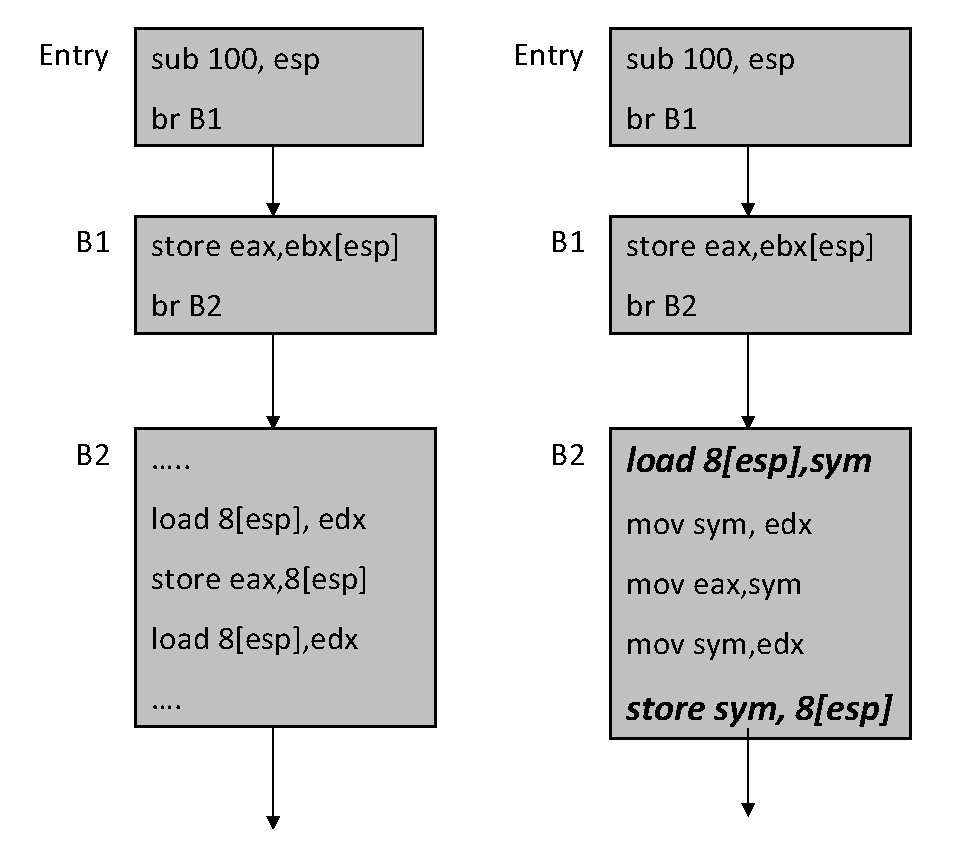
\includegraphics [width=0.5\linewidth] {figures/EPS/cfgex.eps} 
%\tiny{
%\caption { \textit{Stack layout in a binary}}
%}
%\label{fig:stack-layout}
%\end{figure}

\begin{figure}[t]
{
%\begin{minipage}{.5\linewidth}
{
\centering
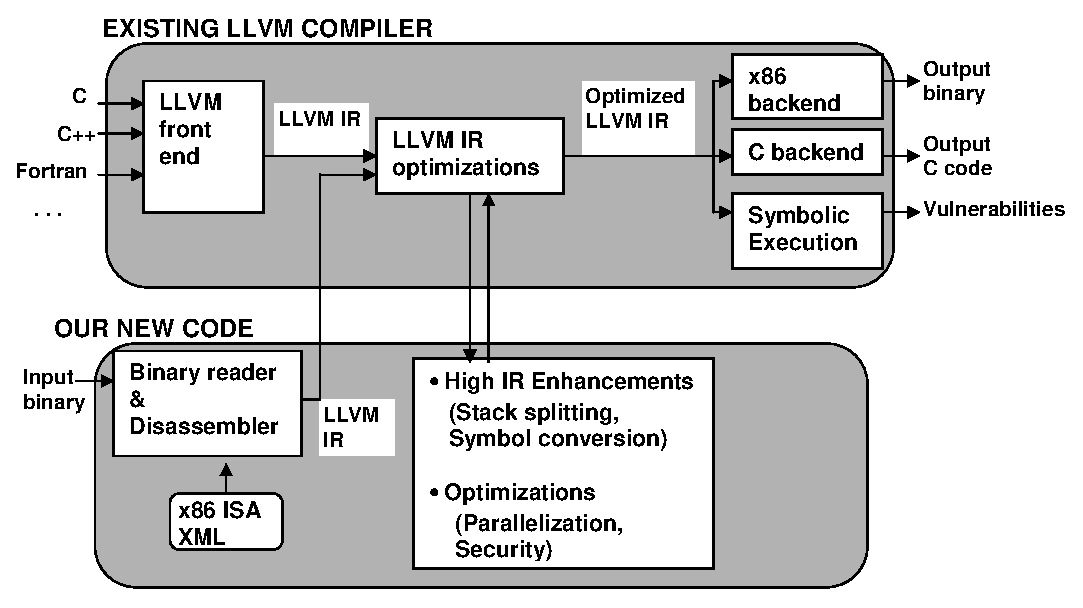
\includegraphics[width=0.7\linewidth]{figures/EPS/flow1.eps}
\caption{\scriptsize{System Flow}}
\label{fig:systemflow}
\vspace{-0.2in}
}
%\end{minipage}
\hfill
%\begin{minipage}{0.3\linewidth}
%{
%\centering
%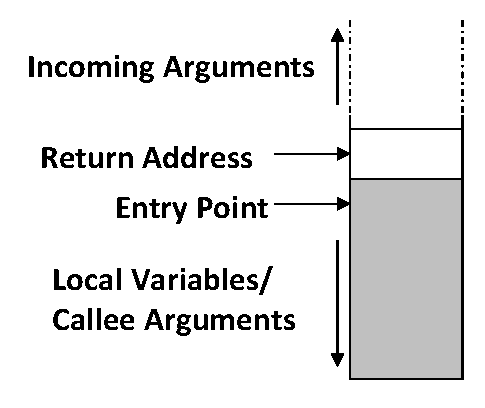
\includegraphics[width=\linewidth]{figures/EPS/stackLayout1.eps} 
%\caption{A typical stack layout}
%\label{fig:stacklayout}
%}
%\end{minipage}
\vspace{-0.2in}
}
\end{figure}

Fig~\ref{fig:systemflow} presents an overview of the \emph{SecondWrite} system. SecondWrite produces LLVM IR using our custom binary reader modules. SecondWrite can be used as a binary rewriter by using the x86 back-end, or as a binary $\rightarrow$ C converter by using LLVM's existing C back-end.
%The frontend module in \emph{SecondWrite} system, consisting of a disassembler and a custom reader module, processes the individual instructions in input executable and generates an initial LLVM IR. This initial representation is devoid of the desired IR features like abstract stack frame and symbols. This initial IR is analyzed to obtain an improved IR which has all the information and features mentioned previously. The standard suite of LLVM optimizations and various new optimization passes can be applied on the above IR to get an optimized IR. The optimized IR is finally passed to the existing LLVM code generator to obtain the rewritten binary. The C backend present in LLVM compiler can be used to obtain C code for better analysis of executables.
%\footnote{Indirect calls and branches occurring in the original binary are handled by translating their target addresses in relocation tables when present in the binary, or through a custom binary rewriting technique we are developing when such tables are absent. However, the choice of technique is orthogonal to the techniques presented in this paper and does not affect our analysis}. 




%\mysection{Decompilation to high-level compiler IR} \label{sec:high-IR}
%\vspace{-2ex}
\section{Deconstruction of physical stack frames} \label{sec:deconstructFrame}
%Binary Stack

%Small description of what next paragraphs are describing
In order to recover a source-level stack representation, we first recognize the local stack frame of a procedure and represent it as a local variable in the IR. As explained in Sec~\ref{sec:contributions}, this local variable is coupled with the rest of the stack due to interprocedural accesses. We achieve this decoupling by recognizing interprocedural accesses and replacing them with symbolic accesses to the procedure arguments. Below, both these techniques are presented in detail. 

%However, this local variable is not decoupled from the rest of the stack given the layout restrictions. For example, procedures access incoming arguments from their parent's stack frame. If the parent frame and the current frame are decoupled and are no longer contiguous, memory accesses to incoming arguments no longer point to their correct locations. We achieve this decoupling by recognizing accesses to the procedure argument space, and replacing them with symbolic accesses to the procedure arguments. Below, we present the detailed description of both of these techniques.

\subsection{Representing the local stack frame} 

We begin by finding an expression for the maximum size of the local stack frame in a procedure X. We analyze all the instructions which can modify the stack pointer, and find the maximum size, P, to which the stack can grow in a single invocation of procedure X among all its control-flow paths. P need not be a compile-time constant; a run-time expression for P suffices when variable-sized stack objects are allowed. An array ORIG\_FRAME of size P is then allocated as a local variable at the entry point of procedure X in the IR.
%The P-byte space includes all the stack frame contents including register spills, callee arguments, and caller and callee-save values. The stack can grow deeper due to calls made by X; however, that allocation is considered as part of callee functions. 

The local variables for the frame pointer and stack pointer are initialized to the beginning of ORIG\_FRAME at the entry point of procedure X. Thereafter, all the stack pointer modifications -- by constant or non-constant values -- are represented as adjustments of these variables. Allocation of a single array representing the original local frame guarantees the correctness of stack arithmetic inside the procedure X.

In some procedures, it might not be possible to obtain a definite expression for the maximum size of the local stack frame. For example, scoped variable-sized local objects in source code might result in a stack allocation with a non-constant amount, whose expression is not available at the beginning of the procedure. Consequently, a single array ORIG\_FRAME of a definite size cannot be allocated. Neither can multiple local arrays, one per such stack increment, be allocated since IR optimizations and compiler backend can modify their relative layout thereby invalidating the stack arithmetic. In such procedures, we do not convert the physical stack 	to an abstract frame. A physical stack frame is maintained in the IR using inline assembly versions of all the stack modification instructions while the remaining instructions are converted to LLVM IR. The runtime checks mechanism presented in the next section is employed to distinguish the local and ancestor accesses. 
%We have found this case of scoped variable-sized stack objects to be exceedingly rare; indeed they did not appear in our benchmarks.
%In such scenarios, the stack frame size and the stack pointer in the caller procedure needs to be adjusted accordingly. Apart from the explicit stack pointer modification instructions inside a procedure, a procedure call might also modify the stack pointer in a way that persists beyond its return.


\begin{figure*}[t]
{
\vspace{-0.2in}
%\centering
{
\begin{minipage}[t]{.44\linewidth}
{
\centering
\begin{scriptsize}
\begin{tabbing}

xxx\=xxxxx\=xxxxxxx\=xxxxxxxxxxx\=  \kill\\

1.\ \ function foo:\\
2.\> \>sub 100, esp   \>\>// Subtract 100 from sp \\
3.\> \>call bar   \>\>// call bar \\
\\
4.\ \ function bar: \\
5.\>\> sub 10, esp  \> \>// Subtract 10 from sp \\
6.\>\> lea  4(esp),edi  \> \>//Move address esp+4 to edi \\
7.\> \>mov  2, ebx   \> \>// Move value 2 to ebx\\
8.\> \>mov  15, ecx  \> \>// Move value 15 to ecx\\
9.\>\> if (esi $\leq$ 5) jmp B2 \>\>//Conditional Branch\\
\\
10.\>B1:\> mov 4,ebx \>\> // Move value 4 to ebx\\
11.\>\> mov 16,ecx \>\> //Move value 16 to ecx\\
\\\
12.\>B2:\> store 10, ebx[edi] \>\>// Store 10 to indirect offset (edi + ebx)\\
13.\>\> store 10, ecx[esp] \>\>// Store 10 to indirect offset (esp + ecx)\\
14.\>\> store 10, edx[edi] \>\>// Store 10 to indirect offset (edi + edx)\\
...
\end{tabbing}
\end{scriptsize}
\vspace{-.2in}
\caption {\textit{A small psuedo-assembly code. The second operand in the instruction is the destination}}
\label{fig:argcodeex}
}
\end{minipage} 
\hfill
\begin{minipage}[t]{.5\linewidth}
{
\centering
\begin{scriptsize}
\begin{tabbing}
xxx\=xxxxx\=xxxxx\=xxxxxxxxxxxxxxxxxxxxxxxxxxxx\=xxxx\=xxxxx\=  \kill\\

1.\ \ function foo:\\
2.\> \>ORIG\_FRAME\_FOO=alloca i32, 100 \>\>// Local frame allocation \\
3.\> \>call\> bar(ORIG\_FRAME\_FOO)   \>// call bar \\
\\
4.\ \ function bar(i32* inArg) \\
5.\> \>ORIG\_FRAME\_BAR=alloca i32, 10  \> \>// Local frame allocation \\
6.\> \> edi = ORIG\_FRAME\_BAR+4 \> \> \\
7.\>\> ebx = 2    \>\>// Move value 2 to ebx\\
8.\>\> ecx = 15    \>\>// Move value 15 to ecx\\
9.\>\> if (esi $\leq$ 5) jmp B2\\
\\
10.\>B1:\> ebx = 4    \>\>// Move value 4 to ebx\\
11.\>\> ecx = 16    \>\>// Move value 16 to ecx\\
\\
12.\>B2:\> store \> 10, ebx[edi]  \>// Store 10 to local frame\\
13.\>\> store \> 10, (ecx-SIZE-BAR)[inArg]  \>// Ancestor Store\\
14.\>\> if((edx+edi - ORIG\_FRAME\_BAR) $\leq$ SIZE-BAR)\>\>\>\>//Run Time Check\\
15 \>\> \>store 10, edx[edi]\>\> //Local Store\\
16.\>\>else\\
17.\>\>\>store 10, (edx+edi - SIZE-BAR)[inArg] \>\>//Ancestor Store\\
...
\end{tabbing}
\end{scriptsize}
\vspace{-.2in}
\caption {\textit{IR of the psuedo-assembly code. SIZE-BAR is size of ORIG\_FRAME\_BAR, register names are pure IR symbols}}
\label{fig:argirex}
}
\end{minipage} 

}
\vspace{-3ex}
}
\end{figure*}
%and have no relation to the hardware register other than their value was in that register name in the input binary
\textbf{Persistent stack modification}: Returns from a procedure ordinarily restore the value of stack pointer to the value before the call. However, in some cases, the stack pointer might point to a different location after returning from a procedure call. For example, the called procedure can cleanup the arguments passed through the stack. To represent this stack pointer modification, which persists beyond a procedure call, we introduce the following definition:\\
\textbf{\emph{Balance Number}}: The balance number for a procedure is defined as the net shift in the stack pointer from before its entry to after its exit. Four different cases can arise:\\
\textbf{Case1}: {\emph{Balance Number} $=$ 0}\\
This is the common case; no modification required.\\
\textbf{Case2}: {\emph{Balance Number} $<$ 0}\\
This case arises when a procedure cleans up a portion of the caller stack frame and is represented as an adjustment of the stack pointer by \emph{Balance Number} amount in the caller procedure after the call. The amount need not be a constant.\\
\textbf{Case3}: {{\emph{Balance Number} $>$ 0}}\\
This case implies that a procedure leaves its local frame on the stack and the corresponding frame outlives the activation of its procedure. Such procedures are represented by considering their allocation as part of the caller procedure allocation. The \emph{Balance Number} amount is added to the size of ORIG\_FRAME array in the caller procedure and the stack pointer is adjusted after the call by this amount. \\
\textbf{Case4}: \emph{Balance Number} Indeterminable\\
In such a case, we do not convert the physical frame into abstract frame and represent the stack as a default global variable in the IR, as shown in Fig~\ref{fig:origCCode}(b). This is an extremely rare case and in fact, it did not appear in our experiments.
%However, the frames in a typical source level IR are active only for the lifetime of the procedure and are automatically deallocated at the exit.

\subsection{Representing procedure arguments} 
\label{sec:procarg}

As per the source-level representation, we aim to represent all the stack-based interprocedural communication through explicit argument framework. We discuss why this is not feasible in all the cases and propose our novel methods based on run-time checks to handle such scenarios. 

%Addressing modes
%Machine-language instruction sets support various addressing modes for accessing stack memory locations: relative addressing via any general-purpose register (x[reg], reg can be esp, ebp or any other register) or generic indirect addressing mode where memory addresses are specified through a register expression such as \emph{base+index$\times$scale+ offset} (where base and index are registers).

%Explanation of VSA
We use Value Set Analysis (VSA)~\cite{gogul04} to aid our analysis. VSA determines an over-approximation of the set of memory addresses and integer values that each register and memory location can hold at each program point. Value Set (VS) of the address expression present in a memory access instruction provides a conservative but correct estimate of the possible memory locations accessed by the instruction. VSA accurately captures the stack pointer modifications and the assignments of stack pointer to other registers.
%VSA is a combined numeric and pointer analysis which determines an overapproximation of the set of memory addresses as well as the set of integer values that each data object (a register or a memory location) can hold at each program point. 

The stack location at the entry point of a procedure is initialized as the base (zero) in VSA and the local frame allocations are taken as negative offsets. Intuitively, memory accesses with positive offsets represent the accesses into the parent frame and constitute the arguments to a procedure. A formal argument is defined corresponding to each constant offset into the parent frame and each such access is directly replaced by an access to the formal argument. 

However, the above method for recognizing arguments is suitable only if VS of the address expression is a singleton set. If the VS has multiple entries, it is not possible to statically replace it with a single argument. We introduce the following definitions to ease the understanding:
{\begin{scriptsize}
\vspace{-0.3ex}
\rule{\linewidth}{0.5pt}\\
{\scriptsize $CURRENT\_BASE$}: Stack pointer at the entry point of a procedure. \\
{\scriptsize $addr_m$}: The address expression of a memory access instruction \emph{m}\\
{\scriptsize $VS(addr_m)$}:Value Set of $addr_m$\\
{\scriptsize $(x,y)$}: Lower and upper bounds, respectively, of the possible offsets relative to {\scriptsize$CURRENT\_BASE$} in {\scriptsize $VS(addr_m)$}\\
{\scriptsize$LOCAL\_SIZE$}: Size of local frame variable {\scriptsize$ORIG\_FRAME$}\\
{\scriptsize$SIZE_{i}$}:Size of {\scriptsize$ORIG\_FRAME_{i}$} of the `ith' ancestor in the call graph, with the caller being represented as the first ancestor. {\scriptsize$SIZE_{0}$} is defined as value 0. \\
\rule{\linewidth}{0.5pt}\\
\vspace{-0.3ex}
\end{scriptsize}}
Fig~\ref{fig:argcodeex} contains an x86 assembly fragment which will be used to illustrate the handling of interprocedural accesses. Fig~\ref{fig:argirex} shows the output IR that results from Fig~\ref{fig:argcodeex}. Three different cases for memory reference categorization of a memory access instruction \emph{m} arise:

\textbf{Case 1} {\scriptsize $(x,y) \subset (-LOCAL\_SIZE,0)$\\}
This condition implies that the current memory access instruction strictly refers to a local stack location. In Fig~\ref{fig:argcodeex}, Line 12 corresponds to this case. Instruction at Line 6 moves address \emph{(esp+4)} to register \emph{edi}. Since the size of current frame in \emph{bar} ({\scriptsize $LOCAL\_SIZE$}) is 10 and the local allocations are taken as negative offsets, this translates to VS of \emph{edi} as \{{\scriptsize $CURRENT\_BASE$-6}\}. The VS of \emph{ebx} at Line 12 is \{2,4\}; therefore the \emph{$VS(dest_m)$} is \{{{\scriptsize $CURRENT\_BASE$ -2 , $CURRENT\_BASE$ - 4}\}, which translates as a subset of (-{{\scriptsize $LOCAL\_SIZE$},0). In this case, we replace the indirect access by an access to the local frame as shown Fig~\ref{fig:argirex} (Line 12).

%Instruction at line 7 moves value 2 to \emph{ebx} and instruction at line 10 moves value 4 to \emph{ebx}. 
  \textbf{Case 2} {{\scriptsize $\exists$ N : $(x,y) \subset (\sum_{i \| i \in (0,N)} SIZE_{i}, \sum_{i \| i \in (0,N+1)}	SIZE_{i})$}\\
This case implies that the current instruction exclusively accesses the local frame of Nth ancestor. In such cases, we make the local frame variable of the Nth ancestor procedure, {{\scriptsize $ORIG\_FRAME_{N}$}, an extra incoming argument to the current procedure as well as to all the procedures on the call-graph paths from the ancestor to the current procedure. The indirect stack access is replaced by an explicit argument access. 
 %It is passed from each procedure to its callee in the call graph as an actual argument until we reach the current procedure. 

Line 13 in Fig~\ref{fig:argcodeex} represents this case. Here, VS of \emph{ecx} is \{15,16\} which translates to the stack-offset range (5,6) which is subset of (0,{{\scriptsize $SIZE_{1}$}). Line 13 in Fig~\ref{fig:argirex} shows the adjusted offset into the formal argument \emph{inArg}. 

%In \emph{bar}, the instruction at line 14 is replaced by an adjusted offset into the formal argument \emph{inArg}, as shown in instruction in line 14 in Fig~\ref{fig:argirex}. 
%The local frame in \emph{foo}, ORIG\_FRAME\_FOO is passed as an actual argument to the procedure \emph{bar}. 

 \textbf{Case 3} \\{\scriptsize 
 $\exists$ N: \{ \{$(x,y) \cap (\sum_{i \| i \in (0,N)} SIZE_{i}, \sum_{i \| i \in (0,N+1)} SIZE_{i}) \neq \phi \} $
 $\wedge$ \{$(x,y) \not \subset (\sum_{i \| i \in (0,N)} SIZE_{i}, \sum_{i \| i \in (0,N+1)} SIZE_{i}) $ \} \}}
			 
This case arises when VSA cannot bound the memory access exclusively to the local frame of one ancestor or to the local frame of the current procedure. It also includes cases where VS of the target location is \emph{TOP} (\ie unknown).
%VSA, being a best effort analysis, can never guarantee a finite value set for every object. Some objects might have a value set TOP, specifying that they can point to any value. In fact, no amount of any advanced static analysis in the executables can assure the discovery of a bounded range for every object. where we cannot distinguish whether the accesses are to the local frame or to some ancestor frame, we insert a run-time check in the IR. This check

We propose a run-time-check-based solution to represent such accesses in the IR. We define all the possible ancestor stack frames in the call graph as arguments to this procedure. Further, at the indirect stack access, a run-time check is inserted in the IR to dynamically translate the access to the local frame or to one of the ancestor stack frames.
% thereafter the value is read from the corresponding location. 

Line 14 in Fig~\ref{fig:argcodeex} represents this case. Suppose $edx$ is data-dependent and hence its VS is $TOP$. Line 14 in Fig~\ref{fig:argirex} shows the run-time check inserted based on this value. Depending on this check, we either access the local frame (Line 15) or the incoming argument (Line 17). 

%An interesting observation helps us in limiting the number of ancestors stack arguments in the above case: an indirect access cannot be to any arbitrary ancestor in the call-graph. An access to a local variable of an ancestor can be made if there is only one path in the call-graph from the ancestor to the current procedure since different paths will have different layouts and compilers cannot know the exact stack layout on all these different paths. This limits the number of ancestors whose arguments need to be passed. The overhead of these runtime checks is likely to be very small since we have found these to be extremely rare in our experiments. 

The cases where {\scriptsize $LOCAL\_SIZE$} is not statically known fall naturally under Case 3. The cases where the stack-frame size in the caller at the point of call is smaller than {\scriptsize $LOCAL\_SIZE_i$}, are handled by considering the actual size at the point of call instead of {\scriptsize $LOCAL\_SIZE_i$}. We have neglected the size of return buffer in our calculations for the ease of understanding. It is easily considered in our model by adding the return buffer size to each ancestor's local frame size.
%The scenarios where the stack-depth in the caller procedure at the time of the call instruction is different from the maximum stack invocation size in the caller procedure, are also easily modeled using the above framework. The details have been suppressed due to the space constraints.
% The incoming arguments are determined by analyzing the offsets into argument space above the local frame space. Since $ebx$ has value set $TOP$, we cannot determine the locations beyond the local frame accessed into argument space; hence, it is not possible to statically determine the number of memory arguments of function \emph{foo}.Any number of new local variables can be added above ORIG\_FRAME in the new stack layout, still providing unrestricted modifications of stack. for this call-site

In the case of dynamically linked libraries (DLLs), the procedure body is not available; hence the above method for handling the arguments cannot be applied. In order to make sure that the external procedures access arguments as before, LLVM code generator is minimally modified to allocate the abstract frame, ORIG\_FRAME, at the bottom of the stack in each procedure in the rewritten binary. Since external procedures are not aware of the call hierarchy inside a program, their interprocedural references are usually limited to only the parent frame. When the prototypes of these external procedures are available (such as for standard library calls), this stack maintenance restriction is avoided altogether by employing the solution presented for any other procedure.
%\vspace{-2ex}
\section{Translating memory locations to symbols}
%\vspace{-2ex}
\label{sec:symprom}
%In x86, the shortage of architectural registers yields an especially large number of memory operations. Promotion of these memory locations to symbols is imperative for effectiveness of traditional compiler analysis in a rewriter. 
Sec~\ref{sec:deconstructFrame} presented methods for deconstructing the physical stack frame into individual abstract frames, one per procedure. Even though this representation allows unrestricted modification of the stack frame, accesses to local variables appear as explicit memory references to locations within this array, which are not amenable to standard data-flow analysis. In this section, we propose our methods for translating these memory operations to symbol operations in the IR.

%\subsection{Limitations of variable identification}
%Commercial disassembly tools like IDAPro~\cite{ida-pro} identify statically determinable stack-frame offsets in the program as local variables. More advanced tools like Divine~\cite{reps06} identify variables from the stack offsets present in the value set of the data objects.
                                                                        
\begin{figure}[t]
{
\vspace{-0.2in}
\centering
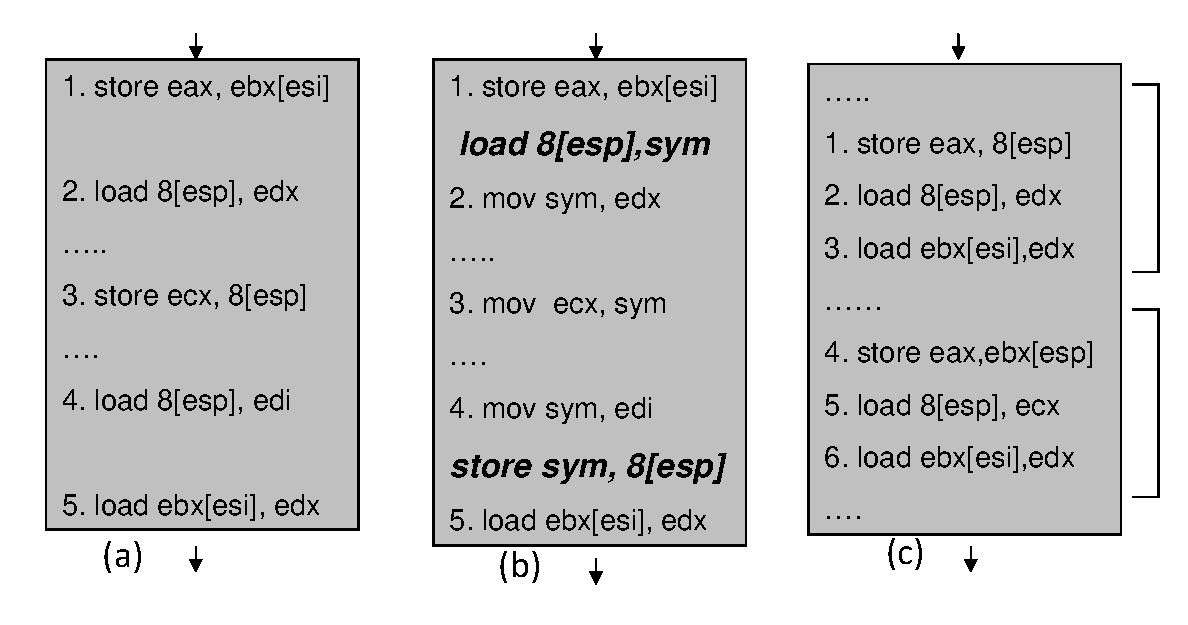
\includegraphics[width=0.7\linewidth]{figures/EPS/pathcfg.eps}
\vspace{-2ex}
\caption{\textit{Symbol promotion. Second operand in the instruction is the destination of the instruction. }}
\label{fig:PromExample}
}
\vspace{-3ex}
\end{figure}






\subsection{Motivation for partitions}

%We need to ensure that the symbol contains the latest data-flow-consistent value for the memory location after any aliasing definition and the memory location contains the latest value consistent with data-flow before we execute an aliasing use. 
As presented in Sec~\ref{sec:contributions}, maintaining the data-flow consistency of the underlying memory locations across the whole program is imperative while promoting memory accesses to symbolic accesses. Fig~\ref{fig:PromExample}(a) shows a small example with three direct accesses to location \emph{(esp+8)} at Lines 2,3,4; the remaining two are unbounded indirect accesses. The simplest method for maintaining the data-flow consistency across the program is to load the data from the memory location into the symbol just after each aliasing definition, store the symbol back to the memory location just before each aliasing use and promote each candidate stack access to a symbolic access, as shown in Fig~\ref{fig:PromExample}(b). The load inserted just after the aliasing definition is referred to as a \emph{Promoting Load} and store just before the aliasing use is referred to as a \emph{Promoting Store} (shown as bold in Fig~\ref{fig:PromExample}(b)). Although this method ensures correct data flow propagation, it results in a large number of promoting loads and stores which might overshadow the benefit of symbol promotion.
%The insertion of promoting loads and stores ensure that the data-flow is maintained correctly and the intermediate direct memory accesses can safely be replaced by symbol accesses. 


\begin{figure}[t]
{
\vspace{-0.2in}
\centering
{
\begin{scriptsize}
\begin{tabular}{|c|c|c|} %|r|r|r|}
%xxxxx\=xxxxxxxxxxxxx\=xxxxxx\=xxxxxxxxxxx\=xxxxxx\=  \kill\\
\hline
\textbf{Statement s}&\textbf{gen[s]}&\textbf{kill[s]}\\ \hline
d:store x,mem[reg]&if([sp+addr]$\in$VS(mem+reg))&if([sp+addr]$\in$VS(mem+reg))\\	
					     &				d 	&				defs(addr) - {d}\\ 
					     &	else \{ \} 	&				else \{ \}\\ \hline
d: store y,addr[sp]&					d	&			defs(addr) - {d}\\ \hline
d: z = load mem[reg]& \{\}&  \{\}\\ \hline
d: z = load addr[sp]&\{\}&	\{\} \\ \hline
\end{tabular}
\begin{tabbing}
Memory location $loc: [sp + addr]$ \\
$mem$: Non-constant access\\
$addr$: Constant\\
$defs(addr)$: Set of instructions defining the memory location [sp+addr]\\
$in[n]$: Set of definitions that reach the begining of node n \\
$out[n]$: Set of definitions that reach  the end of node n \\
$pred[n]$: Predecessor nodes of node n\\
$in[n] = \cup_{i | i \in pred[n]}\{ (out[p])\}$ \\
$out[n] = gen[n] \cup (in[n] - kill[n])$
%\line(1,0){220}
\end{tabbing}
\caption {\textit{The reaching definition description. Definitions are propagated across the control flow of program }}
\label{fig:reachingdef}
\end{scriptsize}
\vspace{-2ex}
}
}
\end{figure}

%Unprofitable case - extra load/stores
Fig~\ref{fig:PromExample}(c) illustrates this unprofitable case. In this example, suppose VS of \emph{ebx} is TOP. Consequently, the instructions at Line 3, 4 and 6 are aliasing indirect accesses to the stack location \emph{(sp+8)}. In order to promote the direct memory accesses at instructions 1, 2 and 5, we need to insert Promoting Stores just before instruction 3 and instruction 6 and a Promoting Load just after instruction 4. Hence, promoting three direct memory operations entails the insertion of three extra memory operations, nullifying the benefit. 

%Need for partition
We propose a novel partition-based symbol promotion algorithm where we divide the program into a set of non-overlapping promotional lifetimes for each memory location. It serves as a fine-grain framework where the symbol promotion decision can be made independently for each lifetime (a partition) instead of the entire program at once. Not doing symbol promotion in a partition does not affect the correctness of the data-flow in the program. The symbol promotion can be selectively performed in only those partitions where it is provably beneficial. Fig~\ref{fig:PromExample}(c) shows an intuitive division of the current example into two safe partitions.

%Partitions are computed based on a reaching definition framework defined on the memory accesses. Next, we present our reaching definition framework for computing the partitions.

\subsection{Reaching definition framework}

We define a new reaching definition analysis on \emph{memory locations} for computing the partitions. This is different from the standard reaching definitions on \emph{symbols} well-known in compiler theory. For each memory location \emph{loc}, this analysis computes the set of instructions defining the memory location \emph{loc} that reach each program point. The set of definitions includes stores to the memory location \emph{loc} using direct addressing mode as well as possibly aliasing stores.

%ValueSet TOP represents that the memory access instruction aliases with any memory location.
Fig~\ref{fig:reachingdef} formulates the reaching definition in terms of VS of the memory accesses. These reaching definitions are propagated across the control flow of the program, similar to the standard compiler dataflow propagation, allowing the partitions to be formed across basic blocks. The interprocedural version of VSA implicitly takes into consideration a local pointer passed to a procedure through an argument.
%For a memory access instruction \emph{m}, we define \emph{$dest_{m}$} as its underlying destination. $ValueSet(dest_{m})$, as determined by VSA, represents the possible memory locations which can be accessed by the memory access instruction \emph{m}.  

\subsection{Symbol promotion algorithm}
%Define DS, Aliasing Loads, Aliasing stores
The candidates for symbol promotion in a procedure P, represented by a set $LOC$, are computed as follows:\\
{\begin{scriptsize}
				 $M$: Set of memory accesses in P\\
				 $DM$: Statically determinable memory accesses, $\bigcup_{d \in M}\{ d | \| VS(addr_{d})\| = 1\}$\\
				 $LOC$: Statically determined stack locations in P, $\bigcup_{d \in DM}\{m | m \in VS(d)\}$\\
				 %$IS$: {Statically undeterminable memory accesses in P} \\
				 	%		 = $\bigcup_{i \in M} \{ i | \|VS(addr_{i}) \| > 1 \vee VS(addr_{i})=TOP \}$ \\
				 %$AS_{m}$: {Indirect accesses aliasing with memory location m} = $\bigcup_{is \in IS}\{is | m \in VS(is)\}$ \\
 \end{scriptsize}}
%,$addr_{m}$: The expression for address of memory access m \\
%Set $DS$ is derived by analyzing ValueSet of underlying destination of each memory access. This allows us to promote even those memory accesses which do not appear as direct stack accesses in binary but nonetheless access only a definite memory location ( e.g ..). The set $IS$ implicitly includes the memory accesses whose ValueSet is TOP.
%\IncMargin{1in}
\begin{algorithm}[t]
{
%\vspace{-0.2in}
%\rule{\linewidth}{1pt}\\
%\begin{tabular}{|c|c|c|}
%\hline
%\end{tabular}
\begin{scriptsize}
 L: Set of loads in P; S: Set of stores in P\\
 DL:$\bigcup_{l \in L}\{ l | \{loc\} = VS(addr_{l})\}$     //Direct Loads \\
 IL:$\bigcup_{l \in L}\{ l | \{loc\} \subset VS(addr_{l})\}$  //Indirect Aliasing Loads\\
 DS:$\bigcup_{s \in S}\{ s | \{loc\} = VS(addr_{s})\}$   //Direct Stores\\
 IS:$\bigcup_{s \in S}\{ s | \{loc\} \subset VS(addr_{s})\}$   //Indirect Aliasing Stores\\
 Processed: Set of elements processed

\While {DS != $\Phi \| $IS != $\Phi$} {
 define new Partition P, define new list $ActiveList$

 \eIf{DS != $\Phi$}{
  s = DS.begin; add s to P.DirectAcc
}{
 s = IS.begin; add s to P.BeginSet
}
add s to ActiveList\\
\While{ActiveList.size!=0}{
s = $ActiveList.top$; Add s to Processed\\
\For{$dl \in DL$}{
\If{s $\in$ in[$dl$]}{
  add $dl$ to P.DirectAcc\\
			\For{$s' \in$ in[$dl$]}{ 
       add s' to $ActiveList$ if s'$\notin$ Processed
}
remove $dl$ from DL
}
}
 \If{$s \in IS$}{
 continue /* No need to store symbol back */
 }
 \For{$il \in$ \{IL,IS\}}{ 
  \If{s $\in$ in[$il$]}{
 add $il$ to P.EndSet}
 \For{$s' \in$ in[$il$]}{ 
 add s' to $ActiveList$ if s'$\notin$ Processed
 }
 remove $il$ from $IL$ if $il \in IL$
 }
 }
 }
\end{scriptsize}
\caption {{{ \textit{Algorithm for computing partitions for a location \emph{loc} in a procedure P}}}}
%\vspace{-2ex}
\label{fig:algpartition}
}
%\rule{\linewidth}{1pt}
%\vspace{-2ex}
\end{algorithm}

Mathematically, for a stack location \emph{loc}, a single partition constitutes three sets of memory accesses: \emph{DirectAcc}, \emph{BeginSet} and \emph{EndSet}. \emph{DirectAcc} contains statically determinable accesses to the location \emph{loc} and constitutes the potential candidates for symbol promotion. \emph{BeginSet} constitutes the indirect stores that may-alias with \emph{loc} and have a control flow path to at least one element of the set DirectAcc. \emph{EndSet} consists of all the aliasing accesses such that there is a control flow path from some element of BeginSet to these accesses. Intuitively, program points just after the elements in BeginSet represent the locations for inserting Promoting Loads. Similarly, program points just before the elements of EndSet are the locations for inserting Promoting Stores. %for loading the latest definition of memory location m to the symbol. 
 %for storing the latest definition of symbol back to the memory location  m. 


%Need to say something about the correctness or optimality of these partitions
%How do we prove that these partitions are correct or optimal?

%Any control flow into a partition is assured to be through either a promoting store or a direct store to the memory location \emph{loc}. The exit is through a promoting load. Even if the symbol promotion is carried inside this partition, the memory location \emph{loc} always has the correct data-flow outside this partition. Consequently, the rest of the procedure is oblivious to the presence of this partition. We first present the method for computing partitions and then provide the benefit-cost analysis for selecting a partition.

%\begin{figure}[t]
{
%\vspace{-0.2in}
\centering
%\psfig{figure=figures/plots/runtimeFinal.eps,width=5.5in} }
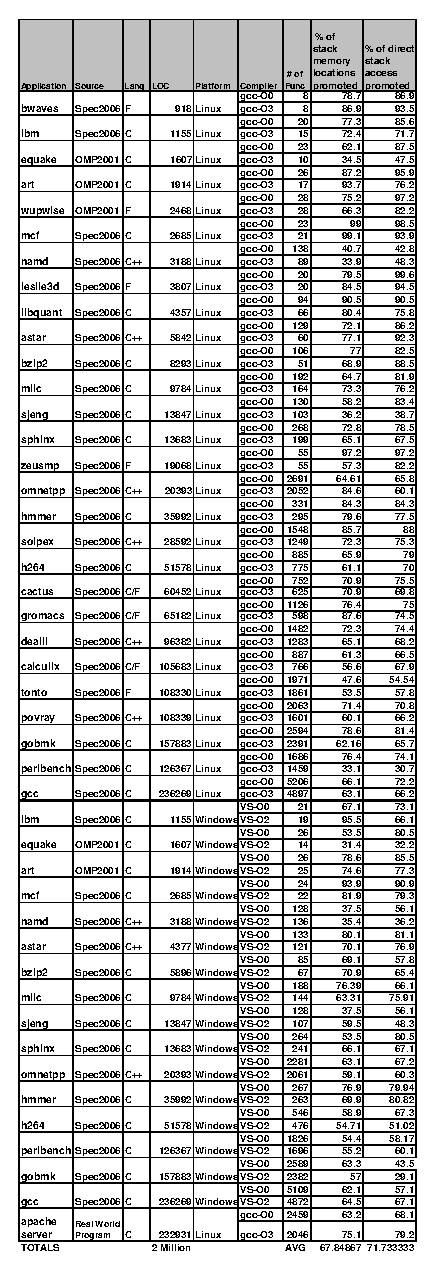
\includegraphics [width=0.7\linewidth] {figures/EPS/appTablenew2.eps} 
%\vspace{-3ex}
\caption { \textit{Benchmarks Table}}
\label{fig:appTable}
}
\vspace{-2ex}
\end{figure}


Algorithm~\ref{fig:algpartition} provides a formal description of the method for computing partitions for a memory location \emph{loc}. We begin with an empty partition. We analyze a store instruction, say \emph{ds}. If \emph{ds} is a direct addressing mode instruction then it is added to the DirectAcc set; otherwise it is added to BeginSet (Line 9-12). Load instructions using direct addressing where \emph{ds} is one of the reaching definitions are added to the DirectAcc set of the partition (Line 16-18). The remaining reaching definitions at these load instructions are added to the analysis list (Line 19-20). If \emph{ds} uses a direct addressing mode, indirect load and store instructions with \emph{ds} as one of the reaching definitions are added to the EndSet (Line 24-26). For indirect stores, the symbol need not be stored back to the memory (Line 22-23). As with the direct loads, the rest of the reaching definitions are added to the analysis list (Line 27-29). This analysis is applied repeatedly until the analysis list is empty. At that point, we have one independent partition. We repeatedly obtain new partitions until there are no more direct stores or indirect stores to analyze. 

We implement a simple benefit-cost model to determine whether the symbol promotion should be carried out for a particular partition. In a partition, the size of DirectAcc set is the number of memory accesses replaced by symbol accesses. We define $Freq_{i}$ as the statically determined execution frequency at program point i. Hence, the benefit of symbol promotion in terms of eliminated memory references:

{\begin{scriptsize}
\begin{equation} 
\begin{split}
Benefit= \sum_{i | i \in DirectAcc}\{ (Freq_{i})\} 
\end{split}
\end{equation} 
\end{scriptsize}}

One promoting load/store is needed for each element of BeginSet and Endset, consequently, the cost:

{\begin{scriptsize}
\begin{equation} 
\begin{split}
Cost= \sum_{i | i \in BeginSet}\{ (Freq_{i})\} + \sum_{i | i \in EndSet}\{ (Freq_{i})\} 
\end{split}
\end{equation} 
\end{scriptsize}}
We calculate the net benefit of each partition as \emph{Benefit - Cost}. Symbol promotion is carried out in a partition only if the net benefit is positive. 


\section{Symbolic Execution}
\label{sec:symExec}

%Introduce symbolic execution
Symbolic execution~\cite{Cadar-EXE} is a well-known technique for automatically detecting bugs and security vulnerabilities in a program. Among various challenges facing symbolic execution, handling symbolic memory addresses (addresses derived from user-input) is an important one. There are two primary approaches for handling symbolic memory. Previous symbolic executors for executables~\cite{Song-Bitblaze, Chipounov-S2E} make simplifying and unsound assumptions by concretizing the symbolic memory reference to a fixed memory location. On the other hand, popular source-level tools like EXE~\cite{Cadar-EXE} and KLEE~\cite{Cadar-KLEE} employ logical constraint solvers to reason about possible locations referenced by a symbolic memory operation. Even though the expressions involving symbolic memory become more sophisticated, these tools outperform the former approaches in terms of path exploration and bug detection.

%The main principle behind this technique is to represent the program inputs with symbolic values instead of concrete input values, and execute the program by manipulating symbolic program expressions. 
%The symbolic expressions along a program path are maintained as a set of constraints. At each potentially vulnerable program point, constraint solvers are employed to check if an input value exists that can trigger an error. The symbolic memory access arises whenever the address in a memory reference instruction is an expression derived from the user input.

\begin{figure}[t]
{
%\vspace{-0.2in}
%\begin{minipage}[t]{0.68\linewidth}
\begin{minipage}{0.68\linewidth}
\centering
{
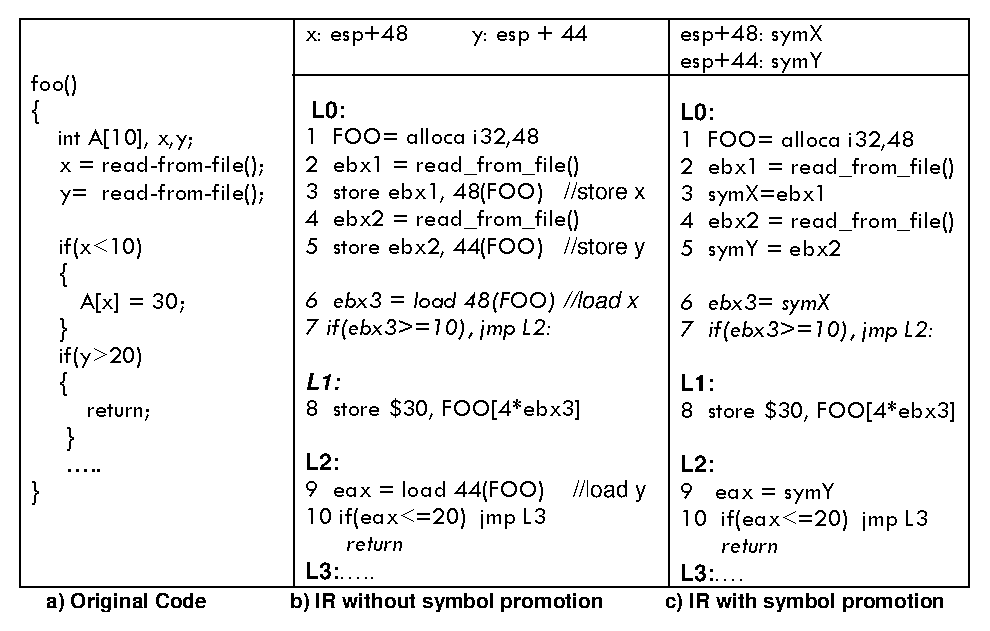
\includegraphics[width=\linewidth]{figures/EPS/symExecution.eps}
\vspace{-2ex}
\caption{\textit{A small source code example}}
\label{fig:symExecSourceCodeEx}
}
\end{minipage}
\hfill
\begin{minipage}{0.3\linewidth}
\centering
{
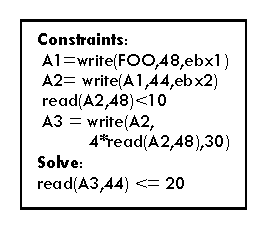
\includegraphics[width=\linewidth]{figures/EPS/symExecConstraints.eps}
\vspace{-2ex}
\caption{\textit{Constraints for Fig~\ref{fig:symExecSourceCodeEx}(b)}}
\label{fig:symExecSourceConstraints}
}
\end{minipage}
\vspace{-2ex}
}
\end{figure}


%Introduce symbolic memory
%, in case any path condition is dependent on an index.  
%One approach is to concretize the symbolic address while the other approach is to simulate a fully symbolic memory.
%Even though these assumptions greatly simplify the subsequent symbolic formulas, it might result in symbolic execution tool to miss some paths.

%\begin{figure}[t]
{
%\vspace{-0.2in}
\centering
%\psfig{figure=figures/plots/runtimeFinal.eps,width=5.5in} }
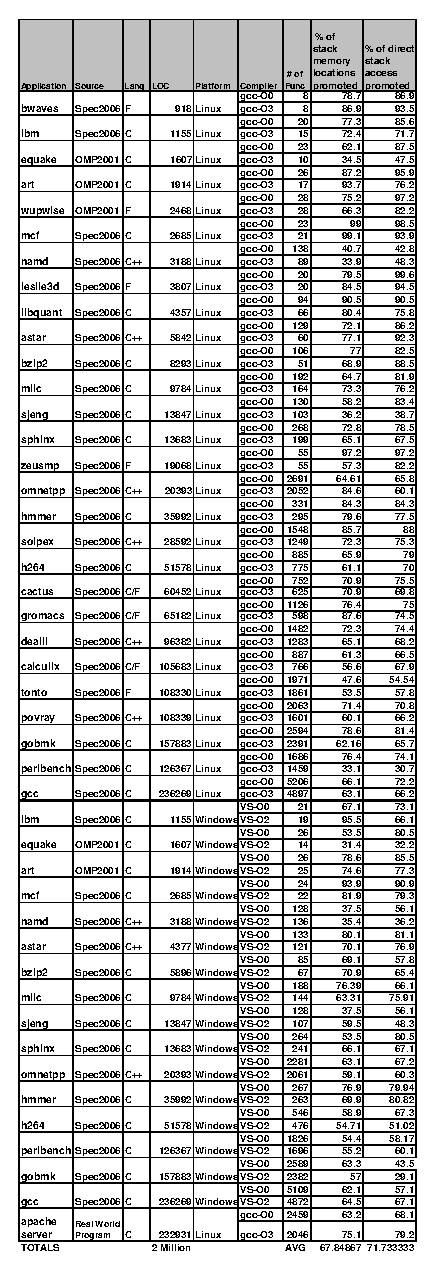
\includegraphics [width=0.7\linewidth] {figures/EPS/appTablenew2.eps} 
%\vspace{-3ex}
\caption { \textit{Benchmarks Table}}
\label{fig:appTable}
}
\vspace{-2ex}
\end{figure}

%Various symbolic execution systems like BitBlaze~\cite{Song-Bitblaze, Chipounov-S2E} make unsound assumptions by concretizing the symbolic memory reference to a fixed memory location. These assumptions greatly simplify the subsequent symbolic formulas obtained while exploring the program paths. However, constraining the memory reference to a fixed location might result in symbolic execution tool to miss some paths, in case any path condition is dependent on an index.  

%Various popular symbolic execution tools like EXE~\cite{Cadar-EXE}, KLEE~\cite{Cadar-KLEE} are based on the latter approach. These tools employ logical constraint solvers to reason about the possible locations referenced by a symbolic memory operation. Even though the program expressions involving symbolic memory are more sophisticated, these tools have been shown to outperform the former approaches in terms of path exploration and bug detection in the programs.

%Why is is more important at binary level
The presence of a physical stack and the lack of symbols in an executable pose a difficult challenge in efficiently extending the logical solver based approach for representing symbolic memory in executables. The most straightforward representation of the memory would be a flat byte array. Unfortunately, the  constraint solvers employed in existing source-level symbolic execution tools would almost never be able to solve the resulting constraints~\cite{Cadar-KLEE}. 

%Some idea about how symbolic promotion solves this challenge
The segmented memory representation in our framework, obtained by abstract stack and symbol promotion, drastically improves the efficiency of such constraint solvers by enabling them to only consider the constraints related to the segments referenced by the current memory address expression and ignore the remaining segments.
% ignore the constraints related to all other segments, thereby, drastically improving their efficiency. 
%In the following discussion, we use the standard notation for representing memory references in case of symbolic execution, where the operation \emph{read(A,i)} returns the value at index i in a  memory array A and \emph{write(A,j,v)} returns a new array with same value as A at all indices except i, where it has value v. Various source level symbolic execution tools map every memory object in the program code to a distinct array. This representation dramatically improves performance since it lets the constraint solvers ignore all arrays not referenced by a given expression. 

Fig~\ref{fig:symExecSourceCodeEx} illustrates this case. Fig~\ref{fig:symExecSourceCodeEx}(a) contains a symbolic memory store to array A. Fig~\ref{fig:symExecSourceCodeEx}(b) and Fig~\ref{fig:symExecSourceCodeEx}(c) show the pseudo IR obtained from an executable corresponding to Fig~\ref{fig:symExecSourceCodeEx}(a), without and with the application of symbol promotion. Fig~\ref{fig:symExecSourceConstraints} shows the constraints and query generated at Line 10 while symbolically executing the path L0$\rightarrow$L1$\rightarrow$L2 in Fig~\ref{fig:symExecSourceCodeEx}(b). Here, \emph{read(A,i)} returns the value at index i in array A and \emph{write(A,j,v)} returns a new array with same value as A at all indices except j, where it has value v.
%\begin{figure}[h]
%\vspace{-3ex}
%\centering
%{
%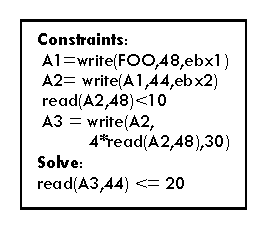
\includegraphics[width=0.3\linewidth]{figures/EPS/symExecConstraints.eps}
%}
%\end{figure}
%\vspace{-3ex}

However, in Fig~\ref{fig:symExecSourceCodeEx}(c), symbol promotion has segmented the array FOO in different segments and references to variables x and y do not refer the segment FOO. Hence, the solver only needs to solve the following simplified query:

{\begin{scriptsize}
\vspace{-2ex}
\begin{equation}
{\scriptsize 
Solve: symY \leq 20
}
\end{equation} 
%\vspace{-2ex}
\end{scriptsize}}
}
%without any constraints
This example only shows the simplification of constraints with symbol promotion. The presence of an abstract stack also results in a similar simplification of constraints by segmenting the memory space within each procedure.

\section{Practical Considerations}
\label{sec:practicalCons}

%General
%Binary Characterization
%Call Translator
%Old segment at same place
%Indirect Branches

\mypar{\underline{Indirect calls and branches}}:SecondWrite implements various mechanisms, as proposed by Smithson et. al.~\cite{matt-patent10}, to address code discovery problems and to handle indirect control transfers. Here, we briefly summarize the mechanism.

A key challenge in binary frameworks is discovering which portions of the code section in an input executable are definitely code. Smithson et. al.~\cite{matt-patent10} proposed \emph{speculative disassembly}, coupled with \emph{binary characterization}, to efficiently address this problem. SecondWrite speculatively disassembles the unknown portions of the code segments as if they are code. However, it also retains the unchanged code segments in the IR to guarantee the correctness of data references in case the disassembled region was actually data. 

SecondWrite employs \emph{binary characterization} to limit such unknown portions of code. It leverages the restriction that an indirect control transfer instruction (CTI) requires an absolute address operand, and that these address operands must appear within the code and/or data segments. The code and data segments are scanned for values that lie within the range of code segment. The resulting values are guaranteed to contain, at a minimum, all of the indirect CTI targets. 
%Binary Characterization generates this list of possible addresses by first constructing a valid address using the base virtual address and the size of the code segment. The code and data segments are subsequently scanned for values that lie within the constructed range. SecondWrite speculatively disassembles the above determined CTI targets as if they are code anyway while also retaining the unchanged segment in case it was data.

The indirect CTIs are handled by appropriately translating the original target to the corresponding location in IR through a runtime translator. Each recognized procedure (through speculative disassembly) is initially considered a possible target of the translator, which is pruned further using alias analysis. The arguments for each possible target procedure (Sec~\ref{sec:procarg}) are unioned to find the set of arguments to be passed to the translator; a stub inside the translator populates the arguments according to the actual target.

%The only way to ensure this is to find a control flow path from the entry point of the execution to that portion. However, the portions of code reachable only through indirect CTIs cannot be discovered statically in all cases. Translators accomplish two major tasks. First, it examines the indirect CTI operand and provide an appropriate adjustment to effectively translate the original address into the corresponding address in the IR. Second,
Above method is not sufficient for discovering indirect branch targets where addresses are calculated in binary. Hence, various procedure boundary determination techniques, like ending the boundary at beginning of next procedure, are also proposed~\cite{matt-patent10} to limit the possible targets.
% For example, function boundary ends at the point at which the next function boundary begins. 
%Various other heuristics are proposed to handle tail calls and multiple entry points.within the current procedure
%If one of the target is outside procedure boundary, it is handled as an indirect call.

\underline{\mypar{Memory Consistency}}:Our framework mimics the assumptions behind all standard software transformation tools with regards to memory consistency. A majority of compilers (gcc, LLVM, Visual Studio) and popular binary frameworks like PLTO~\cite{plto}, DynamoRIO~\cite{bruening2004eta}, PIN~\cite{pintool}, iSpike~\cite{ispike}, Diablo~\cite{Diablo1} reorder code without taking memory consistency into account. Since synchronization is highly multiprocessor specific, most programmers are expected to write synchronized programs using standard synchronization libraries~\cite{SC-compiler}. The presence of synchronization primitives legalizes the applications of all software optimizations.
%The synchronized data accesses are translated to binaries using special synchronization instructions. Hence, the binary optimizers can also safely follow the same compiler model. Our framework also mimics existing software transformation tools about non-preservance of memory consistency in programs. In future work, we can categorize which of our optimizations are not safe under the memory model of target platform and can then turn off the invalid optimizations. for preserving memory consistency by categorizes valid and invalid transformations for each model. 

Recently, the research community is exploring the possibility of preserving memory consistency in software transformation tools~\cite{SC-compiler}. The key idea is to selectively invalidate the transformations for possibly shared memory locations. Currently, our framework can preserve consistency by declaring all possibly shared memory regions as \emph{volatile} in the IR, we plan to work on more detailed  methods in future.
%\emph{thread-escape} analysis in future to minimize the resulting overhead.

{\underline{\mypar{Limitations}}}: Following are the limitations of our current framework, we plan to look at them in future.
\squishlist
\item \textbf{Self Modifying Code}
Like most static binary tools, we do not handle self modifying code. Various tools ~\cite{smc-still} statically detect the presence of self-modifying code in a program. Such a tool can be integrated in our front-end to warn the user and to discontinue further operation.
%However, this is not a serious limitation since most modern operating systems, including Microsoft Windows, prohibit self-modifying code for security reasons~\cite{Win-DEP}. (Note that virtual machines are not self-modifying but rather modify the application, so they pose no problem.) 

\item \textbf{Volatile Memory}
Stripped executables have no information about volatile variables. Existing binary tools~\cite{plto,bruening2004eta,Diablo1,fx32,cifuentes00,atom} ignore their occurrences, instead, we support most common cases of their occurrences. Externally visible volatile variables appear in dynamic symbol table of executables and memory mapped volatile variables can be detected through system calls like \emph{mmap}. Such variables are declared volatile in IR. Volatile variables for exception handling calls (e.g. \emph{setjmp}) are handled by declaring the abstract frame in the corresponding procedure as volatile. Other usages like lock-free variables fall under the umbrella of memory consistency discussed above.
%We prevent symbol promotion for them to preserve correctness. in multi-threaded applications

\item \textbf{Obfuscated Code}
We have not tested our techniques against binaries with hand-coded assembly or with obfuscated control flow.

\squishend

\begin{figure}
	\begin{center}
	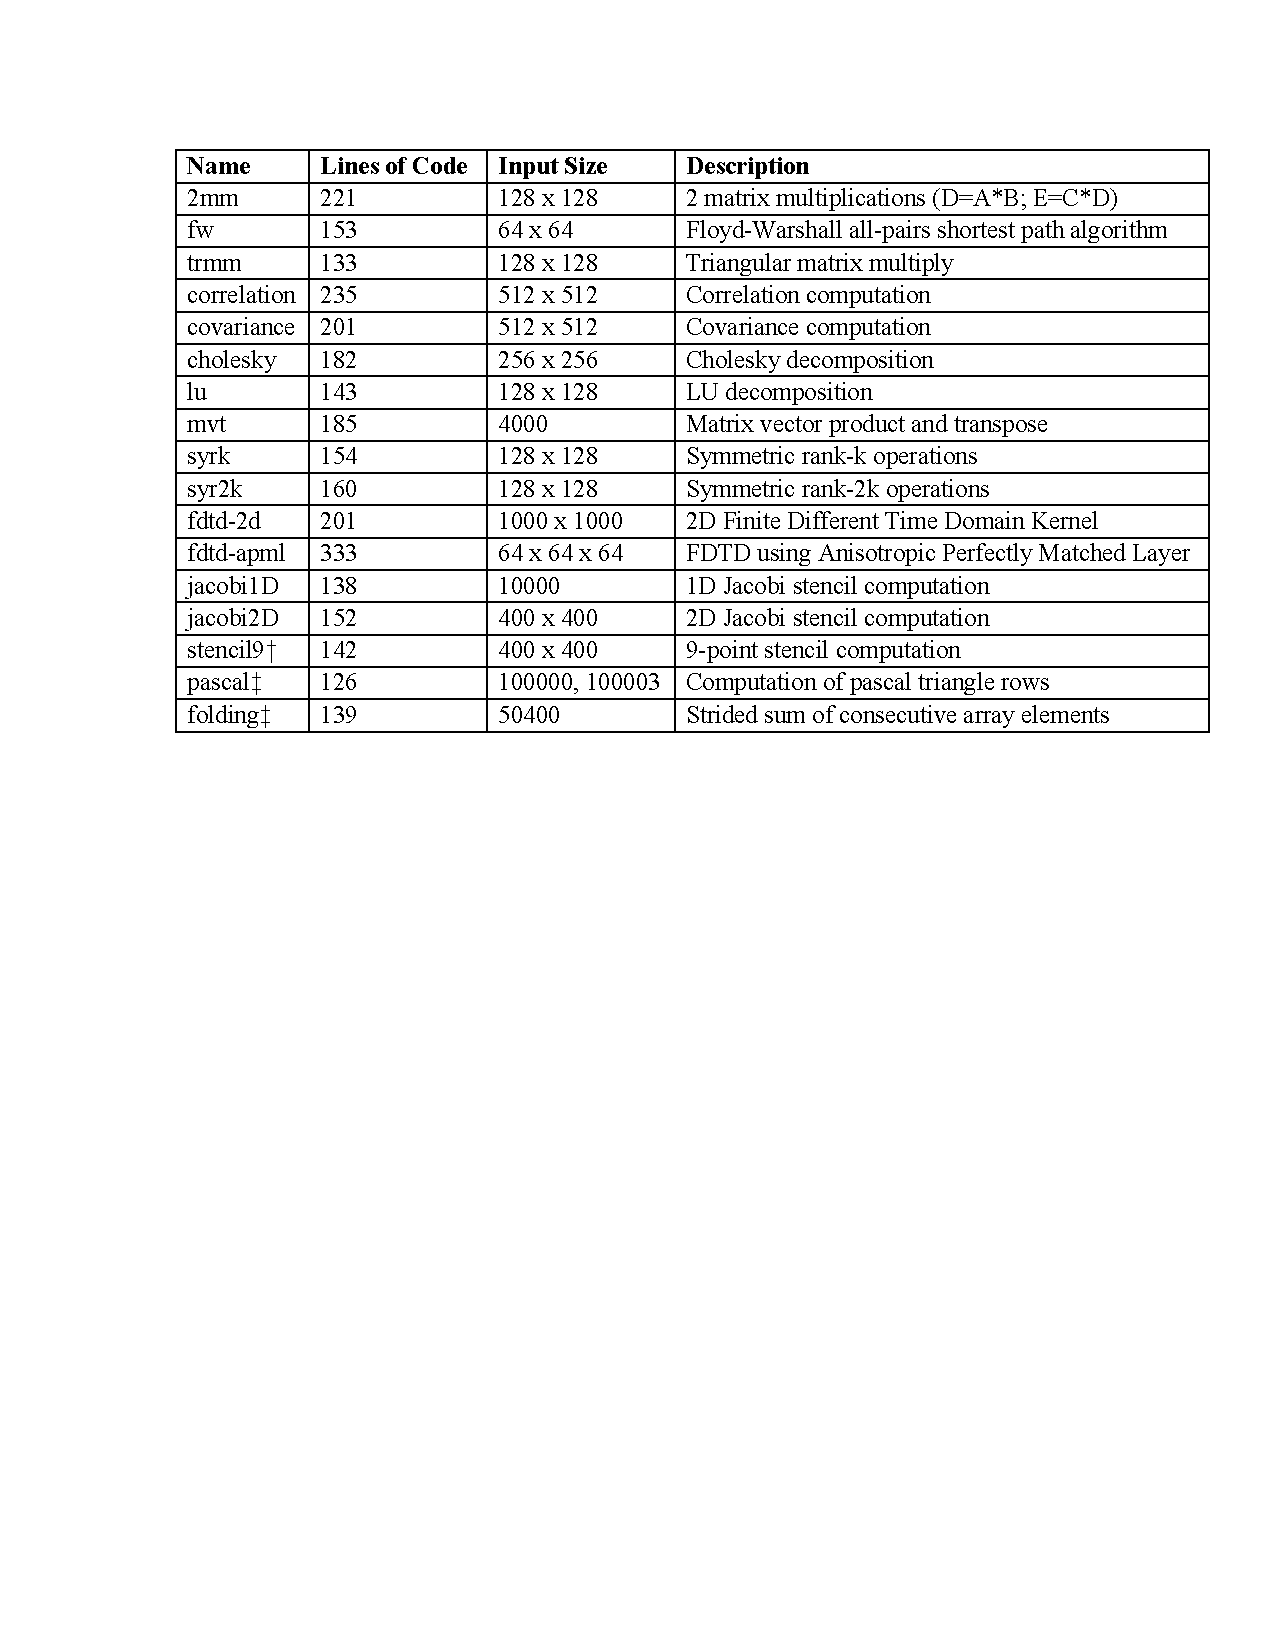
\includegraphics[scale=0.53]{./Figures/Benchmarks.pdf}
	\caption{Benchmark suite. Benchmarks with no symbol after their name were taken from the Polybench suite of benchmarks and translated to Chapel. Benchmarks with $\dagger$ are taken from the Chapel Trunk test directory. Benchmarks with $\ddagger$ were developed on our own in order to test specific data access patterns. }
	\label{benchmarks}
	\end{center}
\end{figure}

\section{Results}\label{sec:results}

To demonstrate the effectiveness of modulo unrolling WU in the Chapel Cyclic and Block Cyclic distributions, we present our results. We have composed a suite of seventeen parallel benchmarks shown in Figure \ref{benchmarks}. Each benchmark is written in Chapel and contains loops with affine array accesses that use zippered iterations, as discussed in \ref{sec:array_slicing}. Our suite of benchmarks contains programs with single, double, and triple nested affine loops. Additionally, our benchmark suite contains programs operating on one, two, and three-dimensional distributed arrays. Fourteen of the seventeen benchmarks are taken from the Polybench suite of benchmarks \cite{polybench} and are translated from C to Chapel by hand. The \textit{stencil9} benchmark was taken from the Chapel source trunk directory. The remaining two benchmarks, \textit{pascal} and \textit{folding}, were written by our group. \textit{pascal} is an additional benchmark other than \textit{jacobi1D} that is able to test Block Cyclic with modulo unrolling WU. \textit{folding} is the only benchmark in our suite that has strided affine array accesses. 

To evaluate improvements due to modulo unrolling WU, we run our benchmarks using the Cyclic and Block Cyclic distributions from the trunk revision 22919 of the Chapel compiler as well as the Cyclic and Block Cyclic distributions that have been modified to perform modulo unrolling WU, as described in Section \ref{sec:adaptation_in_chapel}. We measure both runtime and message count for each benchmark. We also compute the geometric means of all normalized runtimes and message count numbers for both distributions to get a sense on average of how much improvement modulo unrolling WU provided. 

When evaluating modulo unrolling WU used with the Block Cyclic distribution, we could only run two benchmarks out of our suite of seventeen because of limitations within the original Chapel Block Cyclic distribution. Many of our benchmarks operate on two or three-dimensional arrays and all require array slicing for the modulo unrolling WU optimization to apply. Both array slicing of multi-dimensional arrays and array slicing containing strides for one-dimensional arrays are not yet supported in the Chapel compiler's Block Cyclic distribution. Implementing such features remained outside the scope of this work. There was no limitation when evaluating modulo unrolling WU with the Cyclic distribution, and all seventeen benchmarks were tested. Once these missing features are implemented in the Chapel compiler, then our method will apply to all of our benchmarks.

\begin{figure}
	\begin{center}
	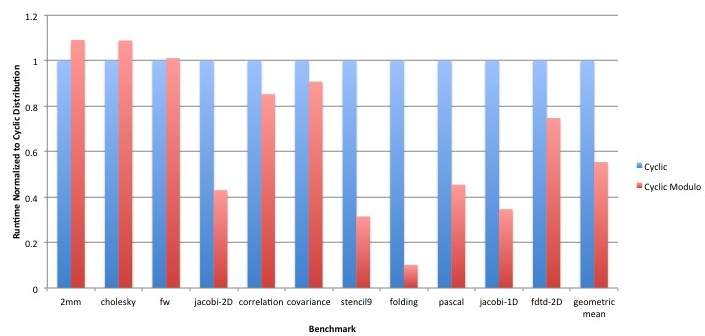
\includegraphics[scale=0.30]{./Figures/cyclic_runtime}
	\caption{Cyclic runtime.}
	\label{cyclic_runtime}
	\end{center}
\end{figure}

\begin{figure}
\begin{center}
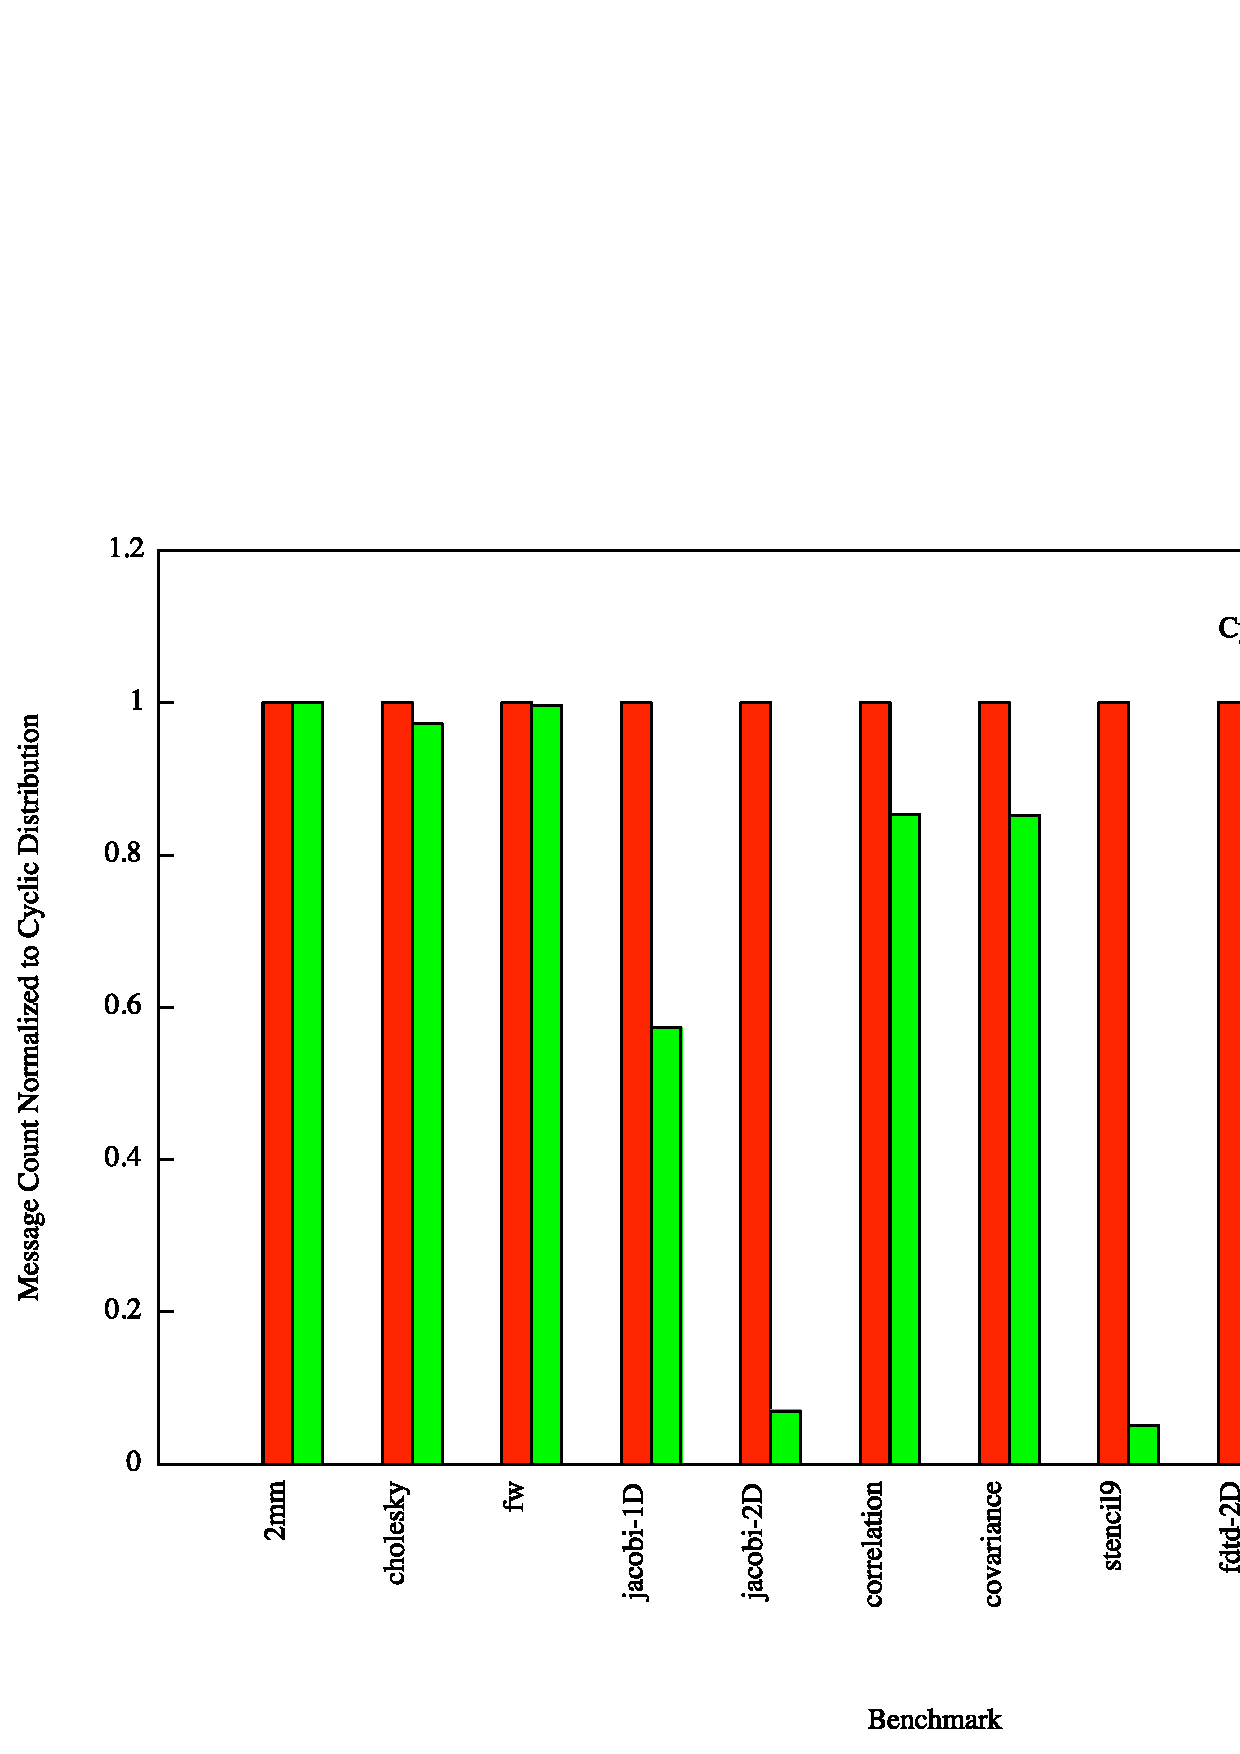
\includegraphics[scale=0.30]{./Figures/cyclic_message_count}
\caption{Cyclic message count.}
\label{cyclic_message_count}
\end{center}
\end{figure}

Figures \ref{cyclic_runtime} and \ref{cyclic_message_count} compare the normalized runtimes and message counts respectively for the Cyclic distribution and Cyclic distribution with modulo unrolling WU. For 8 of the 11 benchmarks, we see reductions in runtime when the modulo unrolling WU optimization is applied. On average, modulo unrolling WU results in a 45 percent decrease in runtime. For 9 of the 11 benchmarks, we see reductions in message counts when the modulo unrolling WU optimization is applied. On average, modulo unrolling WU results in 76 percent fewer messages. 

Some detailed observations on Figures \ref{cyclic_runtime} and \ref{cyclic_message_count} follow. Two of the benchmarks, \textit{cholesky} and \textit{fw}, showed slight improvements in message count when using modulo unrolling WU but did not show improvements in runtime. For the \textit{2mm} benchmark, both runtime and message count did not improve when using modulo unrolling WU. For these benchmarks, the ratio of the problem size to number of locales is not high enough, leading to an insufficient amount of aggregation possible for the computation to see performance improvements. An increase in the number of locales on a system leads to fewer data elements per locale, which naturally means fewer data elements can be aggregated. When this occurs, the cost of performing bulk transfers of a few data elements is more expensive than transferring elements individually. 

\begin{figure}
\begin{center}
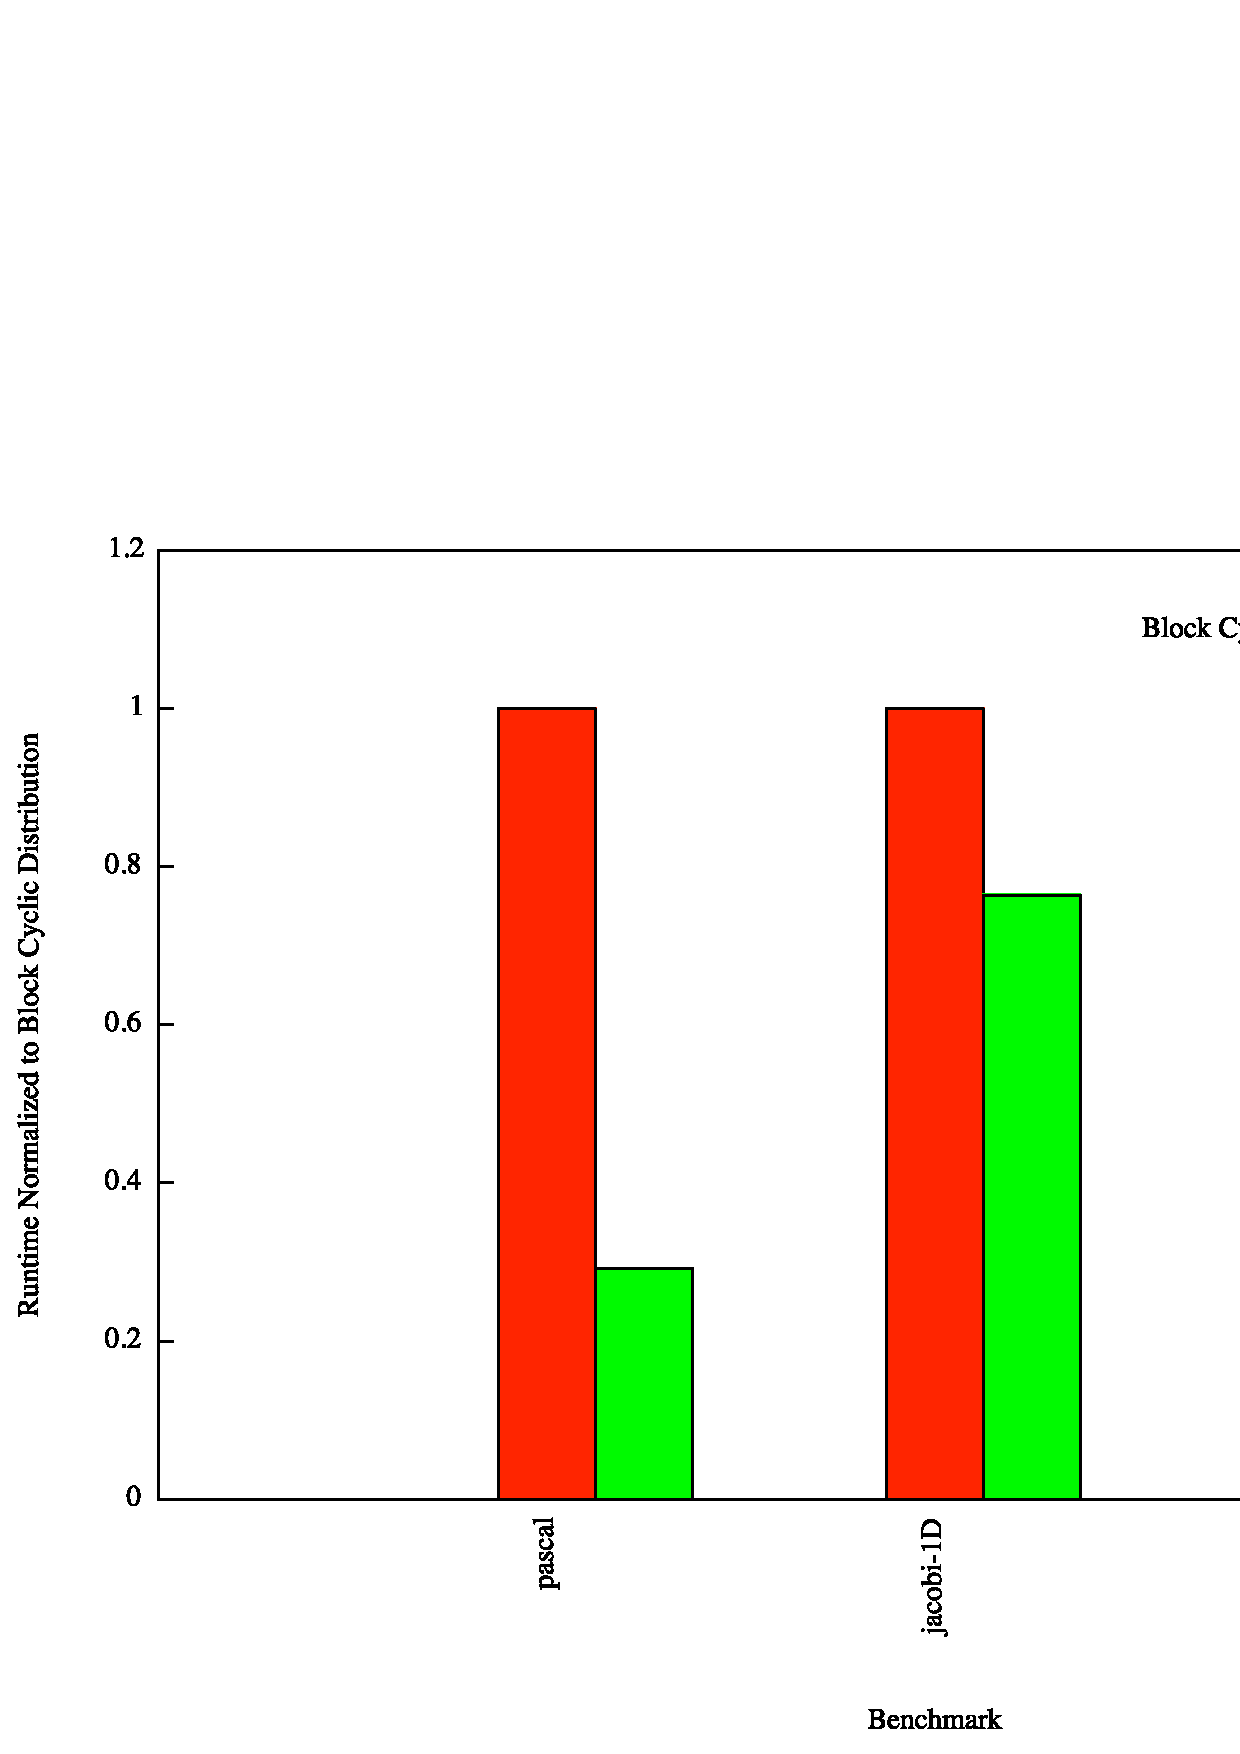
\includegraphics[scale=0.30]{./Figures/block_cyclic_runtime}
\caption{Block Cyclic runtime.}
\label{block_cyclic_runtime}
\end{center}
\end{figure}

\begin{figure}
\begin{center}
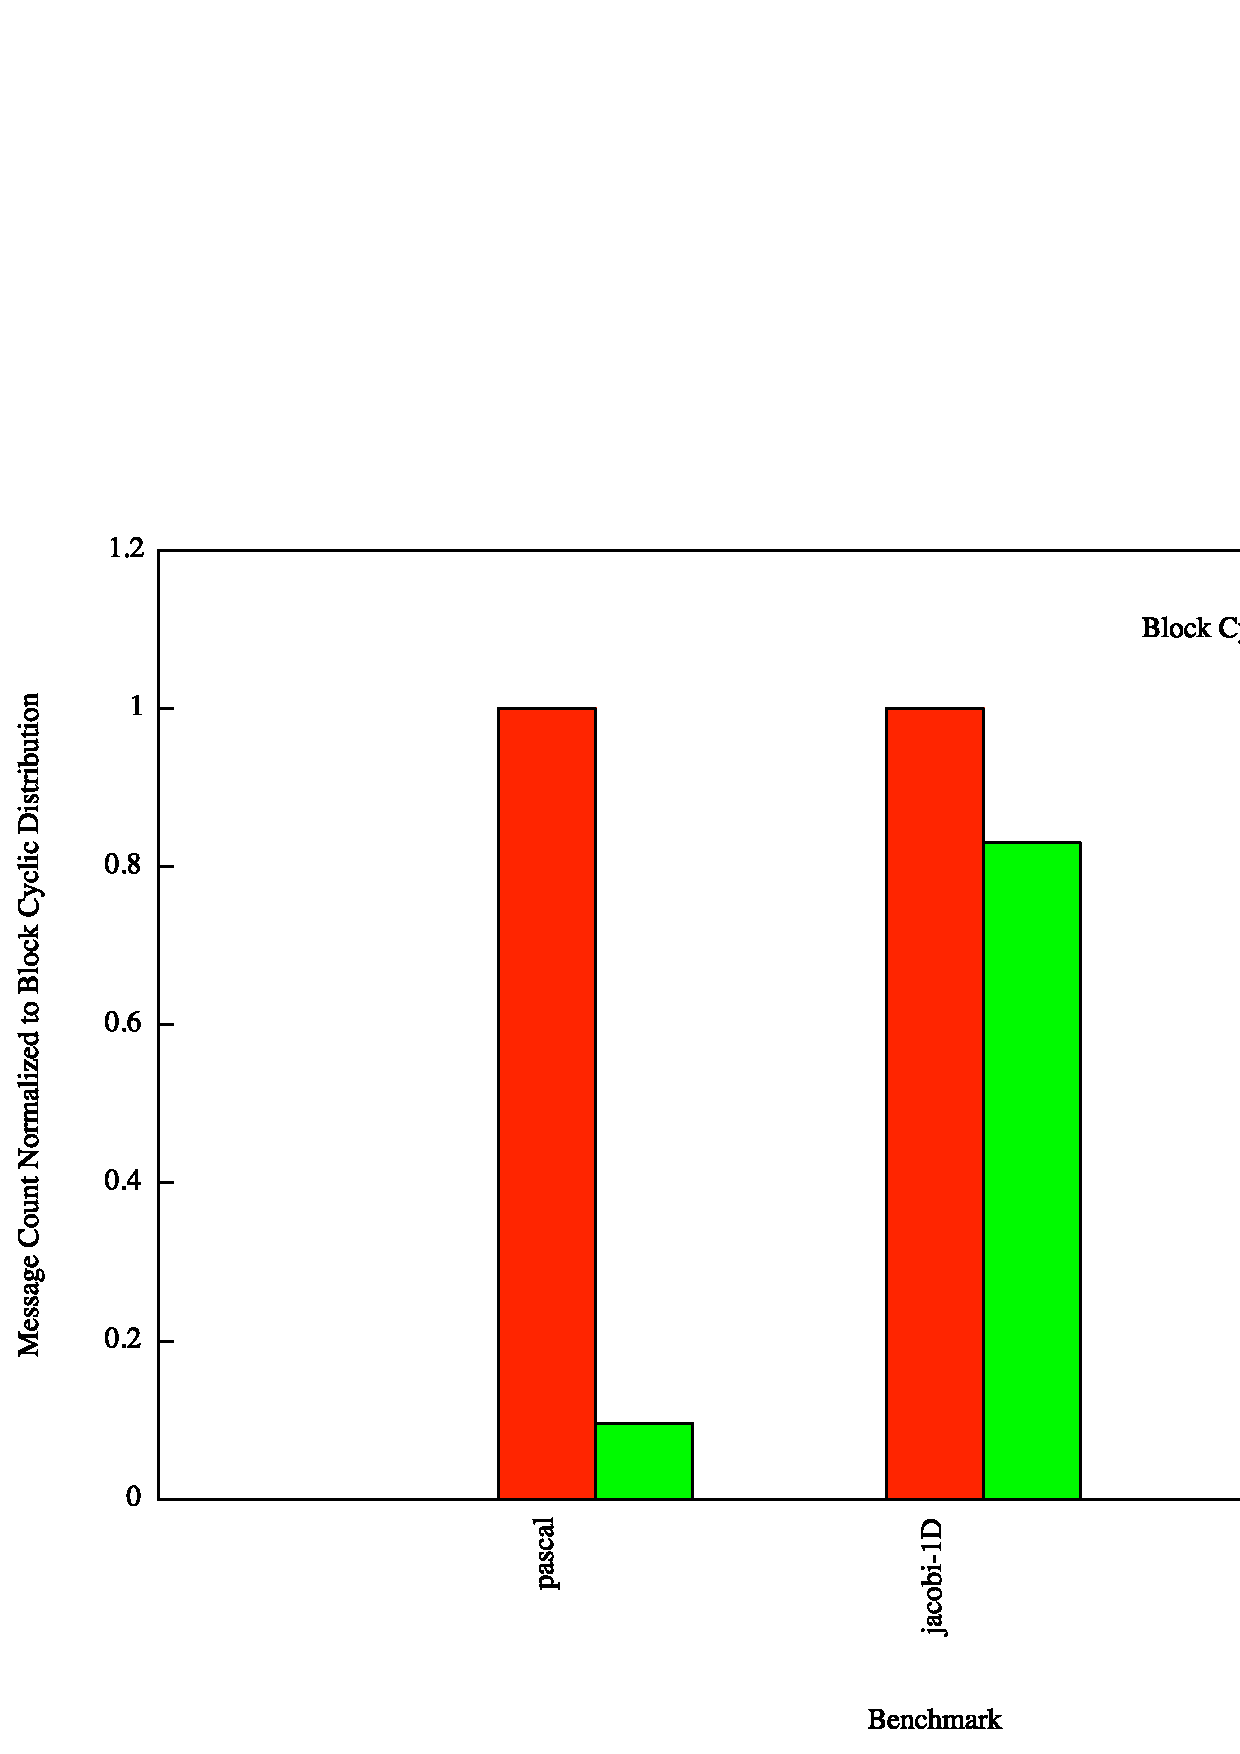
\includegraphics[scale=0.30]{./Figures/block_cyclic_message_count}
\caption{Block Cyclic message count.}
\label{block_cyclic_message_count}
\end{center}
\end{figure}

Figures \ref{block_cyclic_runtime} and \ref{block_cyclic_message_count} compare the normalized runtimes and message counts respectively for the Block Cyclic distribution and Block Cyclic distribution with modulo unrolling WU. For both benchmarks, we see reductions in runtime when the modulo unrolling WU optimization is applied. On average, modulo unrolling WU results in a 52 percent decrease in runtime. For both benchmarks, we see reductions in message counts when the modulo unrolling WU optimization is applied. On average, modulo unrolling WU results in 72 percent fewer messages. 
\vspace{-2ex}
\section{Related Work}
\label{sec:related}
%\vspace{-2ex}
\textbf{Binary rewriting}: Binary rewriting research is being carried out in two directions: static and dynamic. None of the previous dynamic rewriters, PIN~\cite{pintool}, DynInst~\cite{dyninst94}, FX!32~\cite{fx32}, DynamoRIO~\cite{bruening2004eta}, Valgrind~\cite{valgrind} and others, employ a compiler IR. Chipounov~\cite{llvm-qemu} presented a method for dynamically translating x86 to LLVM using QEMU, reporting a huge slowdown of 35x over the baseline QEMU x86-to-x86 translator. Unlike our approach, it converts blocks of code to IR on the fly which limits the application of LLVM analyses to only one block at a time. Further, they do not provide any methods for stack deconstruction or symbol promotion.
% further limiting the effectiveness of optimizations.

%They do not attempt any stack pointer handling or symbols promotion, limiting the effectiveness of these optimizations even further.
% This is not surprising since dynamic rewriters construct their internal representation at run-time, and hence they would not have the time to construct a compiler IR. BIRD~\cite{bird}.  In contrast, we obtain IR for complete binary code at once which allows us to apply complex inter-procedural optimizations.

%Dynamic rewriters are hobbled since they do not have enough time to perform complex compiler transformations either; they have been primarily used for code instrumentation and simple security checks in the past. We do not discuss dynamic rewriters further since this paper's methods are primarily directed at static binary rewriters such as SecondWrite.

% KAPIL: Add Dynamo/RIO to the above list of dynamic rewriters.

Existing static binary rewriters related to our approach include Etch~\cite{newEtch}, ATOM~\cite{atom}, PLTO~\cite{plto}, FDPR~\cite{ibm-fdpr}, Diablo~\cite{Diablo1} and UQBT~\cite{cifuentes00}. All these rewriters define their own low-level custom IR as opposed to using a compiler IR. These IR are devoid of features like abstract frames, symbols and maintain memory as a black-box; the limitations of which have already been discussed in Sec~\ref{sec:intro}. PLTO implements stack analysis to determine the use-kill depths of each function~\cite{plto}. However this information is used only for low-level custom optimizations like load/store forwarding rather than obtaining a high-level IR. UQBT~\cite{cifuentes00} employs function prototypes in its IR, but relies on user to provide this information, instead of determining it automatically from a binary like we do. This severely limits its applicability since only the developers have access to that information.

Virtual machines~\cite{jalapeno-vm} implement stack-walking techniques to determine the calling context by simply iterating over the list of frame pointers maintained as metadata in the dynamic framework; making it orthogonal to our run-time checks mechanism which statically inserts checks in the IR.
%Diablo~\cite{Diablo1} is geared mainly towards optimizations like code compaction for embedded platforms while ATOM is mainly targeted towards RISC architectures like Compaq Alpha. of a procedure invocation, on the stack, dynamic
%Etch~\cite{newEtch} does not explicitly build an IR and allows user to add new tools to analyze and instrument binaries.
 %The primary goal of Etch appears to be instrumentation. 
%, and moreover, the translation process to an intermediate form is no longer automatic.since only the developers have access to that information, and 
%Taking memory as a black box limits its applicability to architectures like x86 which have a limited set of registers. 
%does not attempt to obtain high-level information like function prototypes and  Taking memory as a black box limits its applicability to architectures like x86 which have a limited set of registers. 
%and has only been shown to be applicable for simple optimizations like profile-guided code layout.
%Diablo defines an augmented whole program control-flow-graph-based IR with program registers as globals and memory as a black box. hence it loses out on the advanced set of optimizations implemented in an already existing mature compiler infrastructure.
%UQBT~\cite{cifuentes00} is a binary translation framework which also defines its own custom IR as opposed to using an existing compiler's IR. 
%Ramakrishnan et al~\cite{venki04} suggest static analysis of binaries to check whether coding standards have been followed. which have been employed for different applications. of obtaining information from binaries 

\textbf{Binary Analysis}: King et al.~\cite{dagstuhl-reports-KingMRS12} provide a comprehensive survey of several binary analysis tools. The analysis related to our methods are presented by~\cite{paramRetVal07,gogul04,reps06}. Balakrishnan et al~\cite{gogul04,reps06} present Value Set Analysis for analyzing memory accesses and extracting high level information like variables and their types. As presented in Sec~\ref{sec:contributions}, analyzing variables does not guarantee promotion to symbols in IR. Zhang et al~\cite{paramRetVal07} present techniques for recovering parameters and return values from executables but they do not consider the scenarios where the information cannot be derived.
%Further, their prime aim is to employ this information for security analysis of executables and not for the rewriting.
%Such best effort solutions are good for executable analysis but do not certify the reliable behavior once these analyses fail. Further all these analysis methods have neither been used for the generation of compiler IR nor for any rewriting purposes.

Shastry et al~\cite{shastry-ssa} present methods for register promotion in source programs. Their method relies on memory locations being represented in SSA form with all the aliases exposed, which is a definite non-starter for binaries. Jianjun et al~\cite{dyn-reg-prom11} promote stack variables to registers in a dynamic rewriter, relying on hardware mechanism for memory disambiguation. In contrast, we provide theoretical formulations for symbol promotion without using any hardware support.
%These techniques presented in ~\cite{Cooperregisterpromotion97} are only loop-based methods and are not applicable to binaries since disambiguating memory accesses in binaries is fundamentally different from that in source code. Cooper et al~\cite{Cooperregisterpromotion97} and There have been a lot of tools which employ symbolic execution for detecting vulnerabilities in programs. BAP~\cite{Brumley-BAP},

\textbf{Symbolic execution} : KLEE~\cite{Cadar-KLEE}, EXE~\cite{Cadar-EXE} are example of source-level tools and cannot be applied directly to executables. Previous binary-only symbolic execution tools like BitBlaze~\cite{Song-Bitblaze}, S2E~\cite{Chipounov-S2E} do not represent symbolic memory. MAYHEM~\cite{Brumley-Mayhem} proposes a new index-based memory model for simulating symbolic memory, while our techniques enable application of existing solver based models to binaries.
% without suggesting any new model.Further, these tools achieve symbolic execution only through a dynamic translator like QEMU, limiting its paths to one input, while we achieve symbolic execution in a static translator. 
\vspace{-4ex}
\section{Conclusions}
\label{sec:conclusions}
%\vspace{-1ex}
We present a binary framework which decompiles the input binary into LLVM IR, allowing the application of source-level complex transformations and advanced symbolic execution strategies on executables and enabling functional source-code recovery. In future, we plan to extend our framework for various platform-specific optimizations.
%Our x86 results show that SecondWrite accelerates unoptimized binaries by 27\% on average for our benchmarks, and maintains the performance of already optimized binaries without any custom optimizations.


%\begin{singlespace}
%\begin{scriptsize}

{
%\def\bibfont{\footnotesize}
%\bibliographystyle{ieee}
\begin{singlespace}
%\begin{scriptsize}
%\begin{footnotesize}
\vspace{-3ex}
%\bibliography{angelos,references,local,extra,nghi,kiran,matt,mincy,kiran2,RewriterSurveyReferences,karan,selfmod}
\bibliography{angelos,references,local,extra,matt,mincy,RewriterSurveyReferences,selfmod}
\vspace{-2ex}
\bibliographystyle{abbrv}
%\bibliography{matt}
%\end{scriptsize}
\end{singlespace}
}

%\setlength{\bibspacing}{\baselineskip}
%\bibliography{angelos,references,local,extra,nghi,kiran,matt,mincy,kiran2,RewriterSurveyReferences,karan,selfmod}
%\bibliographystyle{plain}
%\end{scriptsize}
%\end{singlespace}
%\newpage
%\pagestyle{empty}
%\input{facilities}

%\newpage
%\pagestyle{empty}
%\input{mentoring}

\end{document}
